\title{Long Reads Alignment}
\author{
        Giulia Guidi$^{1,2}$, Ayd{\i}n Bulu\c{c}$^2$\\
        \small \{gguidi, abuluc\}@lbl.gov\\
        \small $^1$Dipartimento di Elettronica, Informazione e Bioingegneria, Politecnico di Milano, Milan, Italy\\
        \small $^2$Computational Research Division, Lawrence Berkeley National Laboratory, Berkeley, USA\\
   	   }
\date{\today}

\documentclass[11pt]{article}
\usepackage[english]{babel}
\usepackage[margin=0.9in]{geometry}
%\usepackage[latin1]{inputenc}
%\usepackage[dvips]{epsfig}
%\DeclareGraphicsExtensions{.ps,.eps}
\usepackage{subfigure}\usepackage{cite}
\usepackage{cleveref}
\usepackage{cite}
\usepackage[T1]{fontenc}
\usepackage{fancyhdr}
\usepackage[utf8x]{inputenc}
\usepackage{amsmath}
\usepackage{amssymb}
\usepackage{natbib}
\usepackage{longtable}
\usepackage{cleveref}
\usepackage{ltxtable}
\usepackage{adjustbox}
\usepackage{booktabs}
\usepackage{lipsum}
\usepackage{listings}
\usepackage{mathtools}
\usepackage{graphicx}
\usepackage{float}
\usepackage{setspace}
\usepackage{xcolor}
\newcommand\myworries[1]{\textcolor{red}{#1}}
\newcommand{\figureref}[1]{\figurename~\ref{#1}}
\newcommand{\tableref}[1]{Table~\ref{#1}}
\newcommand{\equationref}[1]{Eq.~\ref{#1}}


\begin{document}
\maketitle

\section{Problem Statement and General Overview}\label{intro}

High-throughput sequencing technologies produce a large number of short and low-quality DNA sequences, called \emph{reads}.
These data are used as starting point to reconstruct the whole DNA sequence in a process called \emph{de novo} genome assembly.

Recent advances in this field, such as the Pacific Biosciences Single Molecule Real-Time (SMRT) Sequencing technology, led to higher consensus accuracy, unbiased error distribution and longer reads.
These improvements are crucial to assemble high-quality DNA sequences.
On the other hand, the SMRT technology is prone to an higher error rate with respect to previous sequencing technology, about 15\%.
In general, high error rates lead to a significant computational effort in throwing away useless data.
The presented work proposes a novel approach to select significant data from the input and recognize overlapping reads pairs to reconstruct the whole DNA sequence.

To give a general overview of our idea, let's consider a pair of reads that share a region of length $k$ (k-mer), as shown in \Cref{fig:overview}.
The probability that such region is correclty sequenced on both the reads is approximately $(1-e)^{2 \cdot k}$ (summation of Bernoulli trials), where $e$ is the error rate.
Then, the probability $P(1,L)$ that at least one k-mer out of $L$ consecutive k-mers being correct in both the sequences is:

$$P(1,L) = 1-(1-(1-e)^{2 \cdot k})^{L}$$

Considering an overlapping region $L$ of 300 base-pairs (bp), with $k$ = 17 and $e$ = 0.15, we obtain that $P(1,300)$ is greater than 70\%.
Starting from these consideration, we decided to base our approach on shared k-mers between reads.
However, we have to face the issue derived from having a high error rate. 
As a matter of fact, an error rate equal to 15\% implies that for large genomes, every possible k-mer will be seen at least once, given enough depth ($d$, sequencer parameter).
Consequently, we would need a k-mer look-up table of size $4^{k}$. 
Furthermore, we have to consider at least a $k$ value equal to 17 as, choosing a smaller $k$, k-mers are not even unique in large genomes.
Using $k$ = 15, we can only encode 1 Gbp possibilities whereas, for instance, the $Human$ genome is $3$ Gbp.
To address this issue and identify overlapping regions, we take into account just a reliable set of k-mers.

\begin{figure}
    \centering
    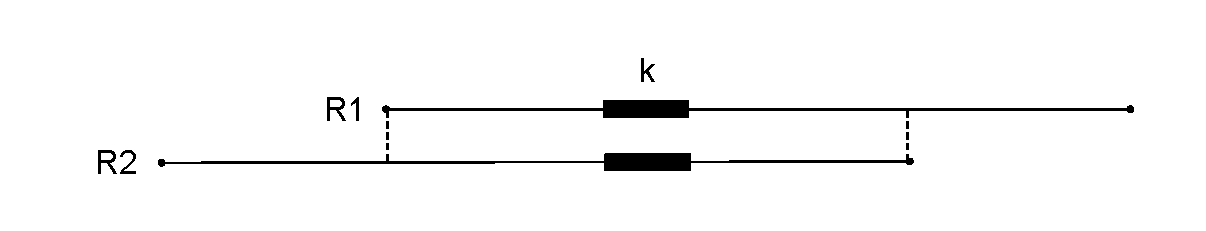
\includegraphics[width=\textwidth]{image/overview.pdf}
    \caption{Pair of overlapping reads sharing a region of length $k$.}
    \label{fig:overview}
\end{figure}
%proposed approach to compute the analysis in Section \ref{code}, while in Section \ref{results} the obtained results are shown.
%In Appendix \ref{append} the raw data used for the final results are reported.

\section{Reliable k-mers}\label{rks}

The first computed analysis regards the identification of a reliable set of k-mers (RKS). 
Our algorithm relies on detecting overlaps between long reads efficiently.
We treat the k-mer occurrences in each long read as the feature vector of that read. 
However, due to high error rates, the number of distinct k-mers in a dataset can be orders of magnitude larger the actual correct k-mers. 
Keeping all the k-mers in our feature set would not only increase the computational costs and memory requirements, it would also lower our precision.

Ideally, we want k-mers that occur only once in the genome. 
Multiple occurences of the same k-mer in the genome correspond to repeat regions. 
If we kept non-unique k-mers in our feature set, they would increase the number of spurious alignments and hence increase the computational costs. 
Our rationale for ignoring non-unique k-mers comes from the observation that either (a) the repeated region is small enough compared to the length of the read that the unique part of the read can still be used to find overlaps of this read with other reads, or (b) that the repeated region is almost as long as the read itself, in which case there is no benefit in aligning this read to other reads because it does not increase our information about the final genome. 

The histogram in \Cref{fig:hist} shows the distribution of unique, non-genomic and repeated k-mers in the genome, given their frequency in the input set of reads.
With $unique$ k-mers we define k-mers that occur only once in the genome, while $non-genomic$ k-mers are those that not exist in the genome and $repeated$ k-mers those that appear multiple times in the genome. 
To obtain the plot, we divide k-mers based on their occurrence in the reads and then, having the reference genome, for each occurrence we compute the amount of unique, non-genomic and repeated k-mers.
We see by looking at the k-mer histogram that the majority of k-mers in the right tail either occur multiple times or do not occur in the genome at all.
Furthermore, \Cref{fig:unique} points out the percentage of unique k-mers over the total amount of k-mers belonging to a certain frequency; the number above each bar represents the absolute number of unique k-mers for a given frequency.
Both \Cref{fig:hist} and \Cref{fig:unique} are obtained using the \emph{Escherichia Coli} genome with $d$ = 30, $k$ = 17 and $e$ = 0.15.
\begin{figure}
    \centering
    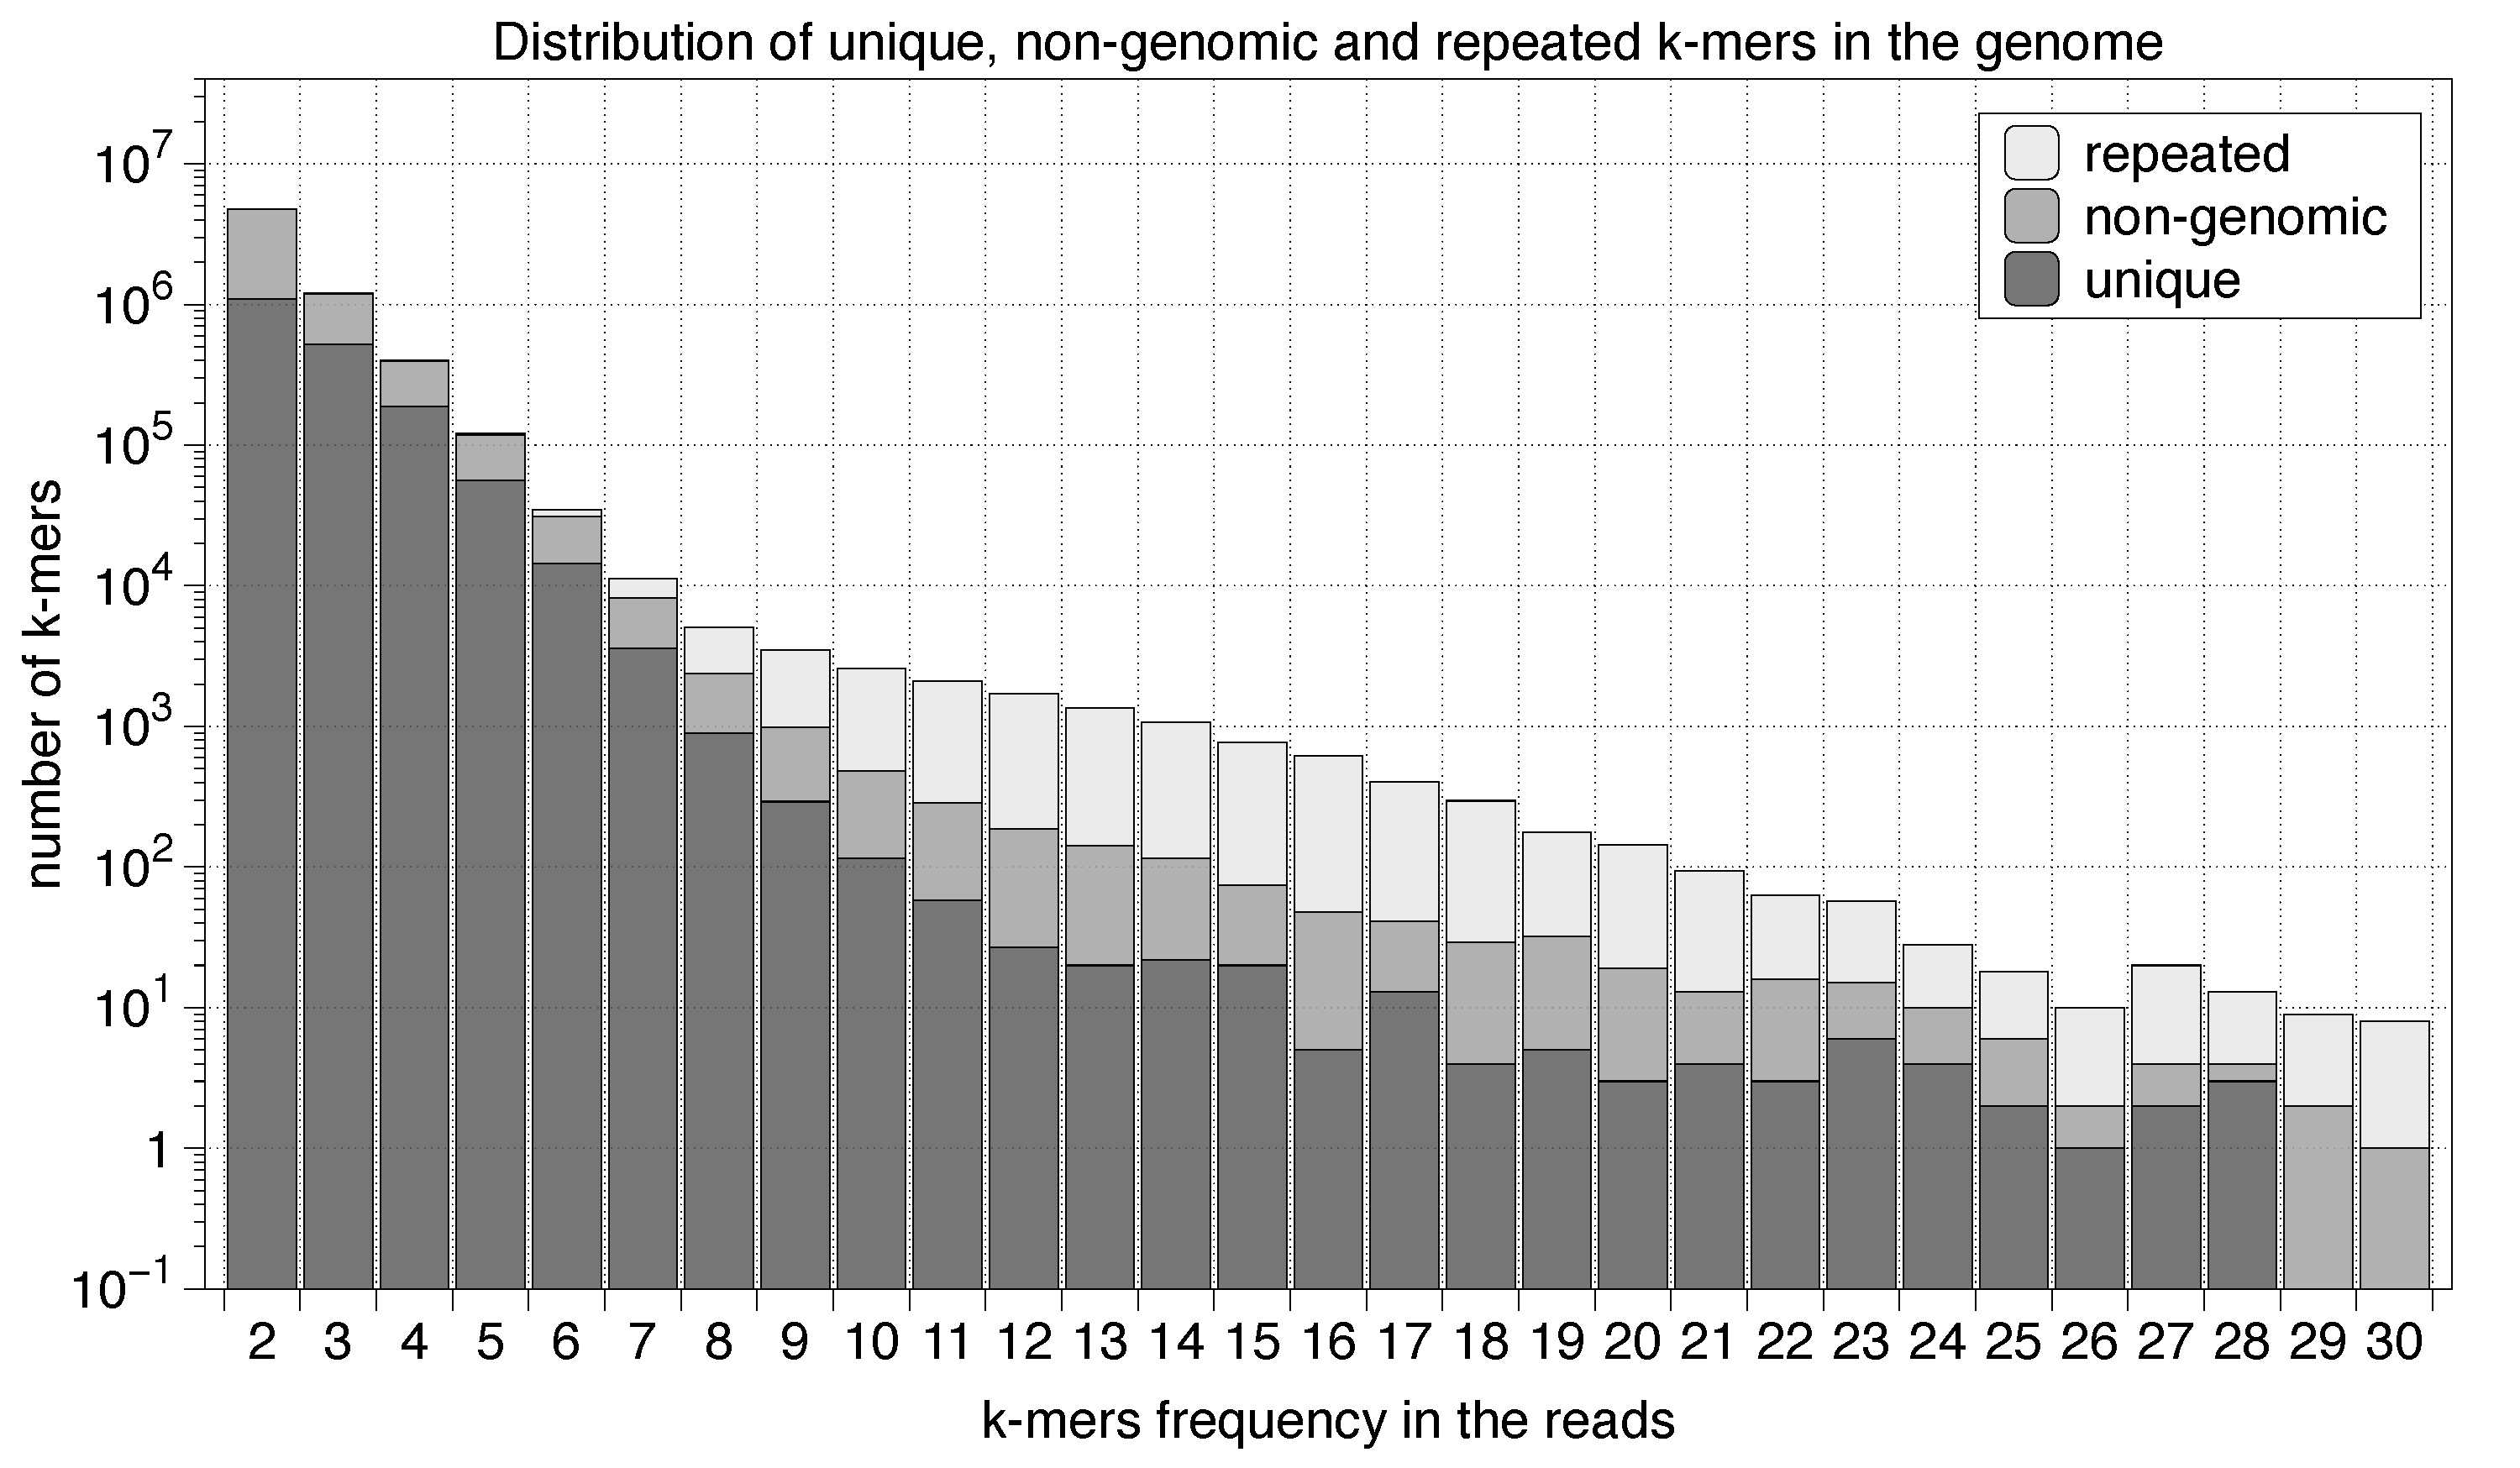
\includegraphics[width=\textwidth]{image/kmerdistribution.pdf}
    \caption{Distribution of unique, non-genomic and repeated k-mers over the total amount of k-mers belonging to a certain frequency.}
    \label{fig:hist}
\end{figure}
\begin{figure}
    \centering
    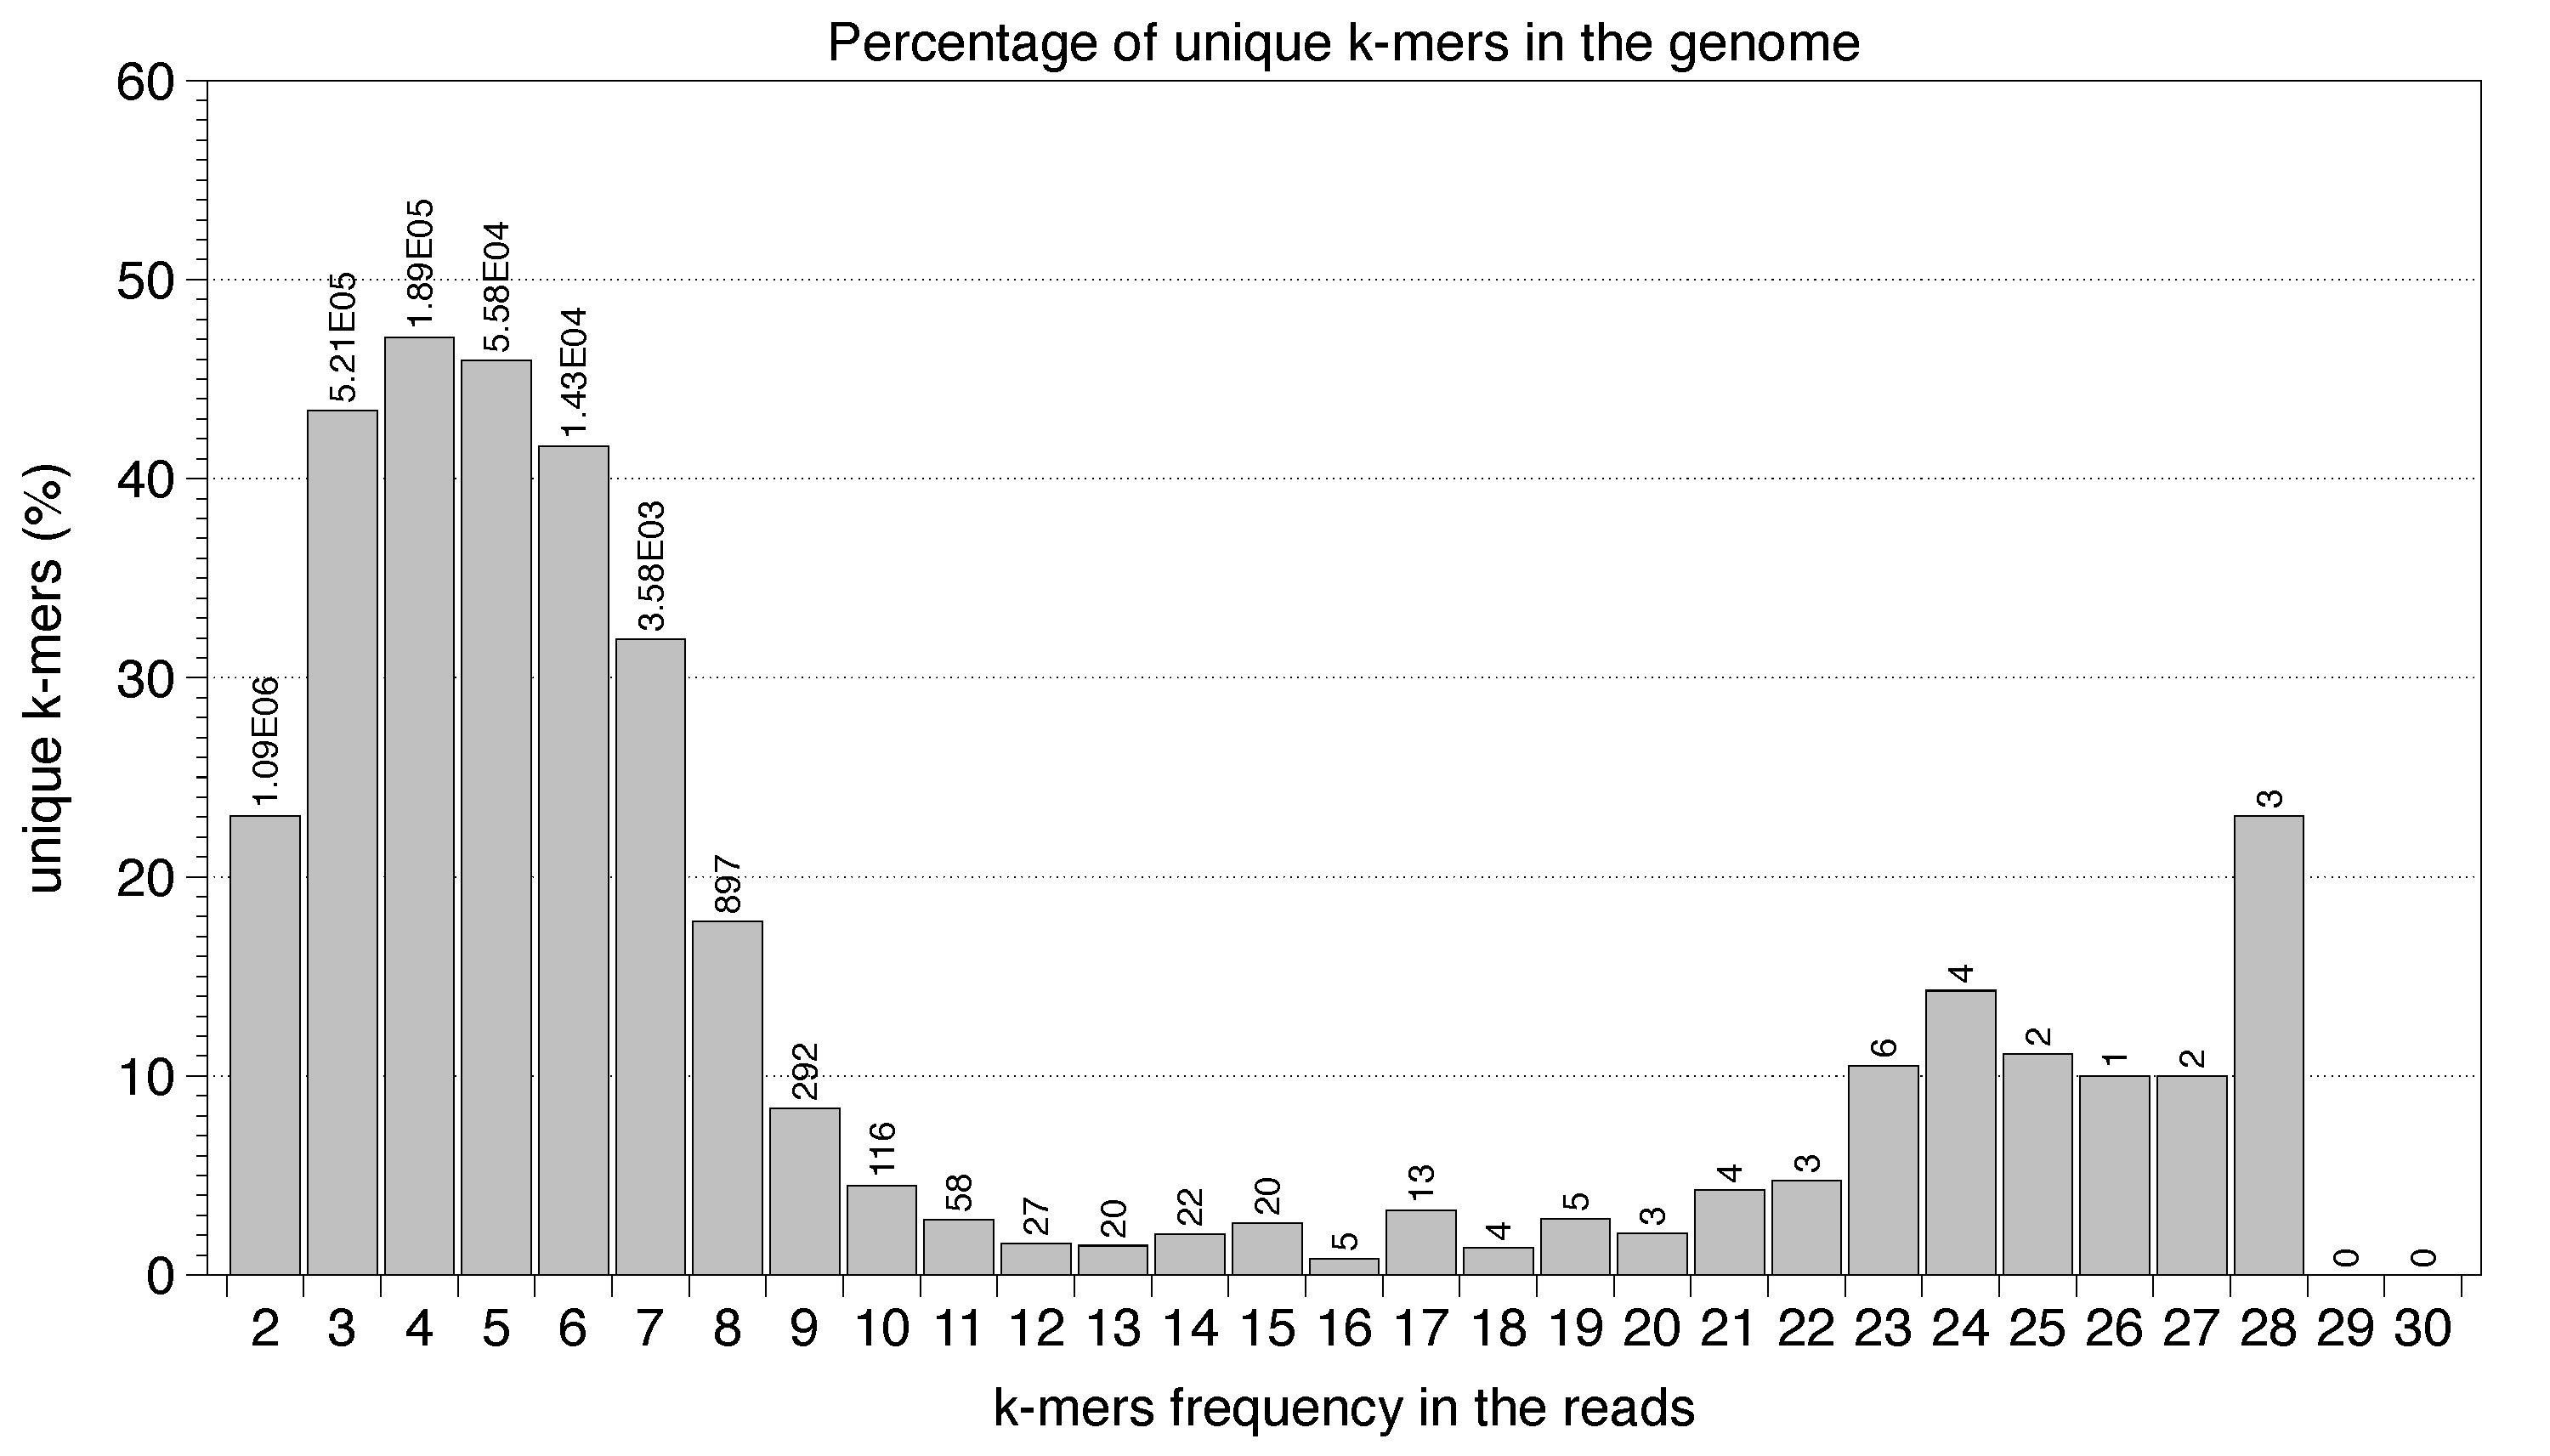
\includegraphics[width=\textwidth]{image/unique.pdf}
    \caption{Percentage of unique k-mers over the total amount of k-mers belonging to a certain frequency. The number above each bar represents the absolute number of unique k-mers for a given frequency.}
    \label{fig:unique}
\end{figure}

The probability of a k-mer being sequenced correctly is approximately $(1-e)^k$ where $e$ is the error rate. If the sequencing depth is $d$, then observing this k-mer in the input data d times  is a very slim $(1-e)^{dk}$. 
Our analysis here is only correct if no other distinct section of the genome has been morphed into this k-mer by error. 
We acknowledge that such morphing occurs in practice but the majority of the high-frequency k-mers in the input set are due to correct sequencing if the value of $k$ is chosen appropriately. 
Take the $Human$ genome that is approximatyely $3$ Gbp and for the sake of argument, only consider substitution errors. 
For $k=17$, it encodes $4^{17}=16$ billion different k-mers. 
Assuming independence, every possible k-mer exists in the genome with probability $3/16$. 
The probability that a 17-mer we have seen being the result of off-by-1 error in sequencing is $(3/16) \cdot 17 \cdot e \cdot (1-e)^{17-1} \approx 3 e (1-e)^{16}$, whereas the probability of sequencing a 17-mer correctly is $(1-e)^{17}$.

The probability that observing a k-mer that corresponds to a unique (non-repetitive) region $d-1$ times in the input would be approximately $P(d-1) = d (1-e)^{(d-1)k} (1-(1-e)^k)$. 
To generalize, the probability to observe $d-t$ times is:

 $$P(d-t) = {d \choose t} (1-e)^{(d-t)k} (1-(1-e)^k)^t$$

\begin{figure}
    \centering
    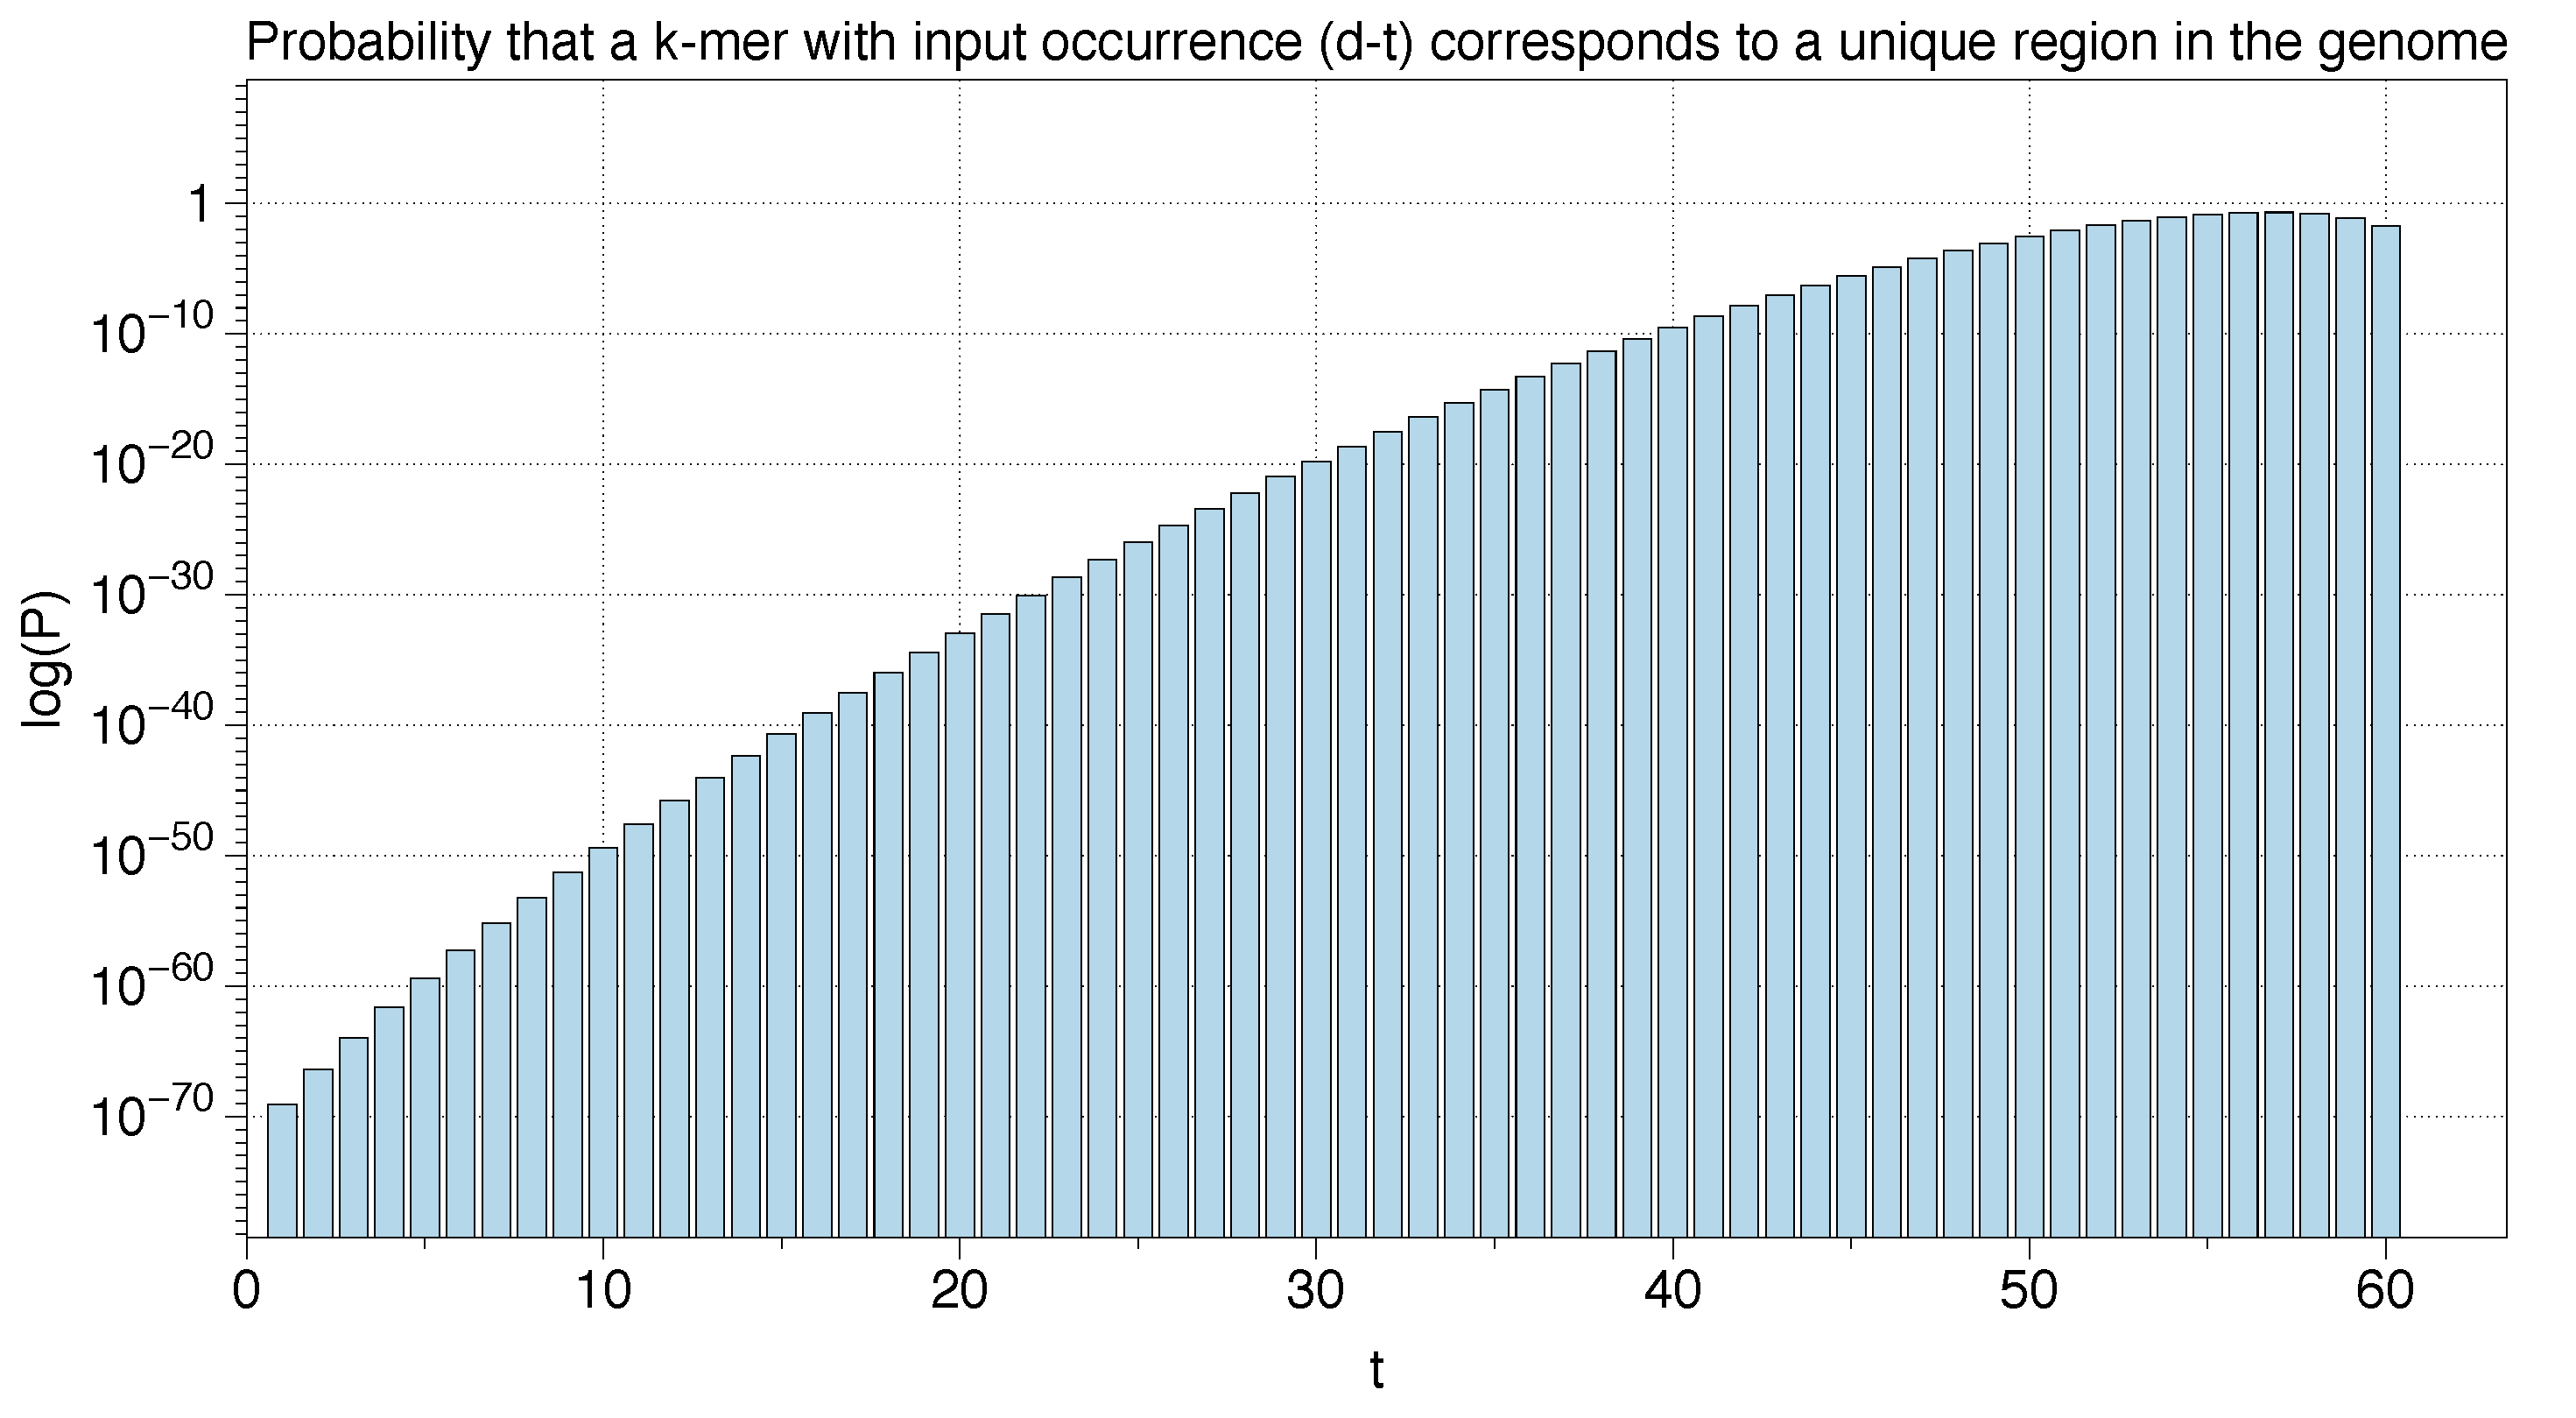
\includegraphics[width=\textwidth]{image/pdt.pdf}
    \caption{Probability that observing a k-mer that corresponds to a non-repetitive region $d-t$ times in the input for
    $d$ = 60, $k$ = 17 and $e$ = 0.15.}
    \label{fig:pdt}
\end{figure}
\Cref{fig:pdt} shows the probability that a k-mer with input occurrence $d-t$ corresponds to a unique region in the genome given $d$ = 60, $k$ = 17 and $e$ = 0.15.
%The reads were generated starting from the Escherichia Coli genome, using the %PacBio reads simulator.
%Then, using Jellyfish software, we generated different k-mers dataset from %these reads, varying the value of \emph{k}, we took into account values from %15 to 29.\\
%The k-mers belonging to the RKS set are chosen looking at their occurrence %among the generated reads..\\
%The following plots (Figure \ref{fig:0}, \ref{fig:1}, \ref{fig:2} and \ref{%fig:3}) show the percentage of RKS over the total number of generated k-mers %per each k-mer occurrence, taking into account different k-mers length.\\
%For the following analysis, we decided to take into account \emph{k} values %equal to 15, 17 an 19.
%\section{Algorithm Approach}\label{code}
%
%The proposed algorithm exploits a trie tree approach to find matches between %k-mers and the genome \cite{bodon2003trie}.
%This approach makes the algorithm much more efficient with respect to its %previous version.
%It takes as inputs the reference genome, the k-mer set generated from it and %the k-mer length (k). 
%The trie is a particular tree datastructure which associates an alphabet to %each node. 
%In a nutshell, the advantage of a trie-based structure is that during the %matching phase the algorithm follows a single path down along the tree, %without matching against each single k-mer.\\
%In our context, the alphabet corresponds to the nucleotides, as shown in %Figure \ref{fig:node}.
%In addition to the four pointers to nucleotides, in this implementation, the %datastruct \emph{node} includes also two integer values: \emph{Count} and \emph%{GroupID}.
%The first one is used during the string matching phase in order to track the %occurence of a match.
%It is incremented only in leaf nodes when a matching is found.
%The second one is used during the building phase; it is associated with each %leaf node and it represents the occurrence in the initial k-mer set of a %specific k-mer.
%Figure \ref{fig:trie} shows an example of trie tree structure based on a 4-mer %set.\\
%Currently, the trie is built based on kmer set.
%However, given that the size of the genome file is smaller than one of the %kmer set, it may make sense to build the trie based on the first one.
%
%\begin{figure}
%    \centering
%    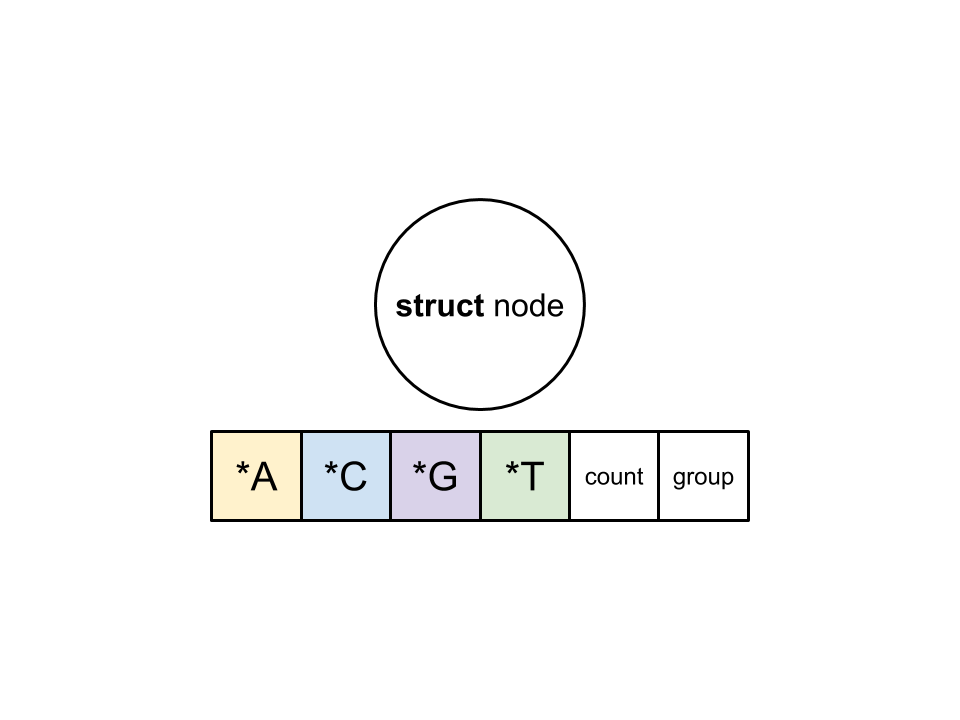
\includegraphics[scale=0.35]{image/TrieNode.png}
%    \caption{Graphical representation of the trie node}
%    \label{fig:node}
%\end{figure}
%\begin{figure}
%    \centering
%    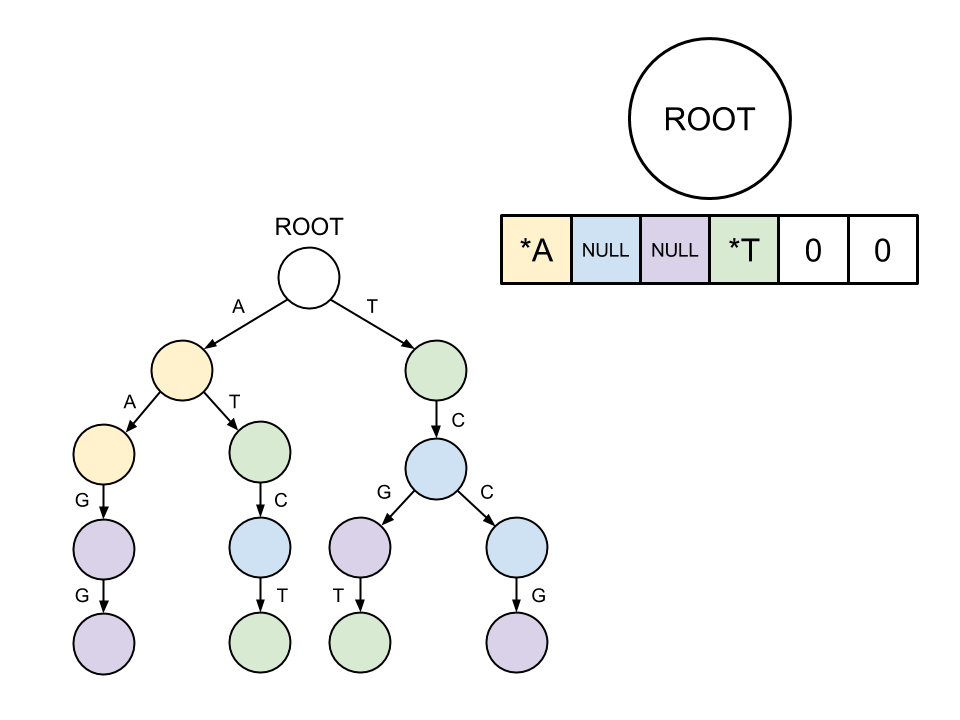
\includegraphics[scale=0.435]{image/TrieStruct.png}
%    \caption{Graphical representation of the trie tree structure for a 4-mer %set}
%    \label{fig:trie}
%\end{figure} 

%\section{Existence and unique existence of k-mers in the genome}\label{%existence}
%
%Here, we computed some statistics con the previously selected dataset of k-mer.
%The goal was to identify which groups of k-mers, based on their occurrences in %the initial dataset (that means the occurrence in the reads generated from the %PacBio simulator), presented the highest percentages of unique existence in %the genome.
%To do that, we found the matches between each k-mers of the dataset and the %genome sequence.\\
%The \emph{GroupID} variable represents the occurrence of a k-mer in the %initial dataset. 
%\emph{State A}, \emph{State B} and \emph{State C} indicate the number of %k-mers (within a group, that means with the same occurence in the initial %dataset) with \emph{real} occurence in the genome equal to 0, equal to 1 and %greater than 1, respectively.
%Regarding the presented plots, for all of them the x-axis is based on the \emph%{GroupID}, while the y-axis represents both the percentage of k-mers existence %and unique existence of k-mers in the genome (Figure \ref{fig:15}, \ref{fig:17}% and \ref{fig:19}).\\
%The percentage of existence (Eq.\ref{eq:first}) and unique existence (Eq.\ref{%eq:second}) are defined as:
%\vspace{5mm}
%
%\begin{equation}
%Existence = \frac{State B + State C}{State A + State B + State C}\cdot 100
%\label{eq:first}
%\end{equation}
%\begin{equation}
%Unique\, existence = \frac{StateB}{StateA + StateB + StateC}\cdot 100
%\label{eq:second}
%\end{equation}
%
%\vspace{6mm}
%\noindent
%Figure \ref{fig:15} shows the obtained results with the k-mer length equal to %15, the \emph{GroupID} goes up to 268.
%The greater unique existence percentages, drawn with red dashed line, are %associated with \emph{GroupID} equal to 5, 6 and 7 (with a maximux of 47.84\% %for \emph{GroupID} equal to 6).\\
%Figure \ref{fig:17} shows the obtained results with the k-mer length equal to %17, in this case the \emph{GroupID} goes up to 166.
%The greater unique existence percentages, drawn with red dashed line, are %associated with \emph{GroupID} equal to 4 and 5 (with a maximux of 48.01\% for %\emph{GroupID} equal to 4).\\
%Figure \ref{fig:19} shows the obtained results with the k-mer length equal to %19, in this case the \emph{GroupID} goes up to 118.
%The greater unique existence percentages, drawn with red dashed line, are %associated with \emph{GroupID} equal to 3 and 4 (with a maximux of 46.69\% for %\emph{GroupID} equal to 4).\\
%In order to compare results with different k-mer length, a maximum \emph{%GroupID} equal to 90 is considered for all the x-axis\footnote{The depth is %equal to 30.}.

%\section{Statistics about reads pairs}\label{pairs}
%
%To figure out how many of the found reads pairs actually belong to the same %region of the genome that means they represent \emph{true overlap}, we %implemented a statistics using the file in MAF format genereted by PacBio %simulator.
%This file contains the alignment position of each reads on the genome.
%From this analysis, we obtained that about the 50\% of the reads pairs found %by our algorithm represent \emph{true overlap}.\\
%\myworries{To do: extend this paragraph and insert plot.}
%Furthermore, we generated an histogram to represent the percentage of pairs %sharing a certain number of k-mers.
%Assuming that pairs sharing few k-mers do not bring significant information, %we decided to delete reads pairs sharing a k-mers number lower than a \%myworries{threshold} starting from the next step of the algorith.

\section{Proposed algorithm}\label{algorithm}

To identify the overlapping reads pairs, the proposed approach exploits sparse matrices.
This because sparse matrices express the data access patterns in a concise and clear manner, allowing better organization of computation and generality.
The column-by-column algorithm we use is equivalent to the k-mer index table concept in HipMer and many other assembler. 
The first step consists in the creation of a sparse matrix where row are represented by the reads and columns by the set of reliable k-mers.
The cell $(i,j)$ contains the k-mer $id$ and the positions of that k-mer in the considered read.
%The ultimate goal of the previous analysis consists in obtaining a [k-mer -by- read] matrix (where $A_{ij}$ is the occurrence/absence of k-mer $i$ in read $j$).
This matrix is used as starting point for the construction of a feature vector in finding alignments among the reads.
Consequently, we create the transpose of the first one obtaining a $kmers-by-reads$ matrix, as shown in \Cref{fig:matrices}.
\begin{figure}
    \centering
    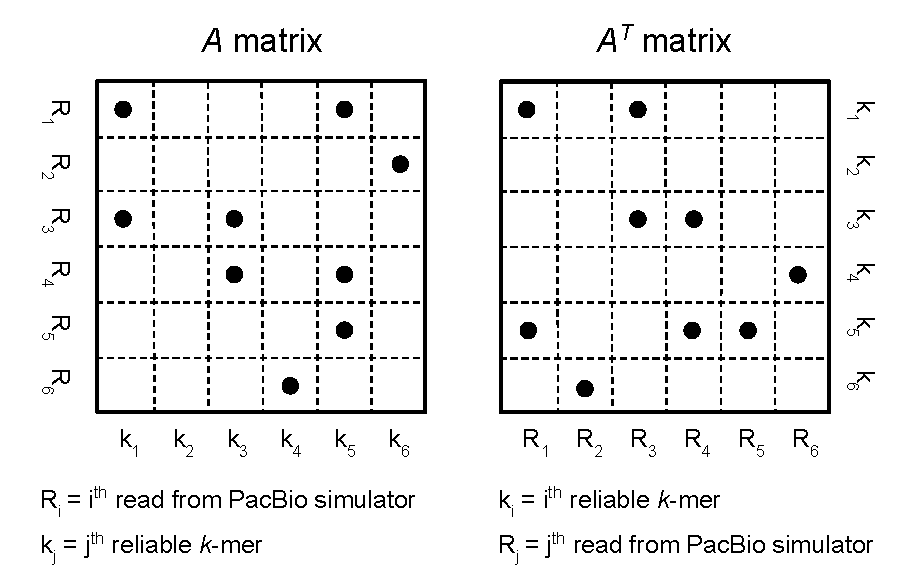
\includegraphics[width=\textwidth]{image/matrices.pdf}
    \caption{Sparse matrix $reads-by-kmers$ on the left and its transpose on the right.}
    \label{fig:matrices}
\end{figure}
\begin{figure}
    \centering
    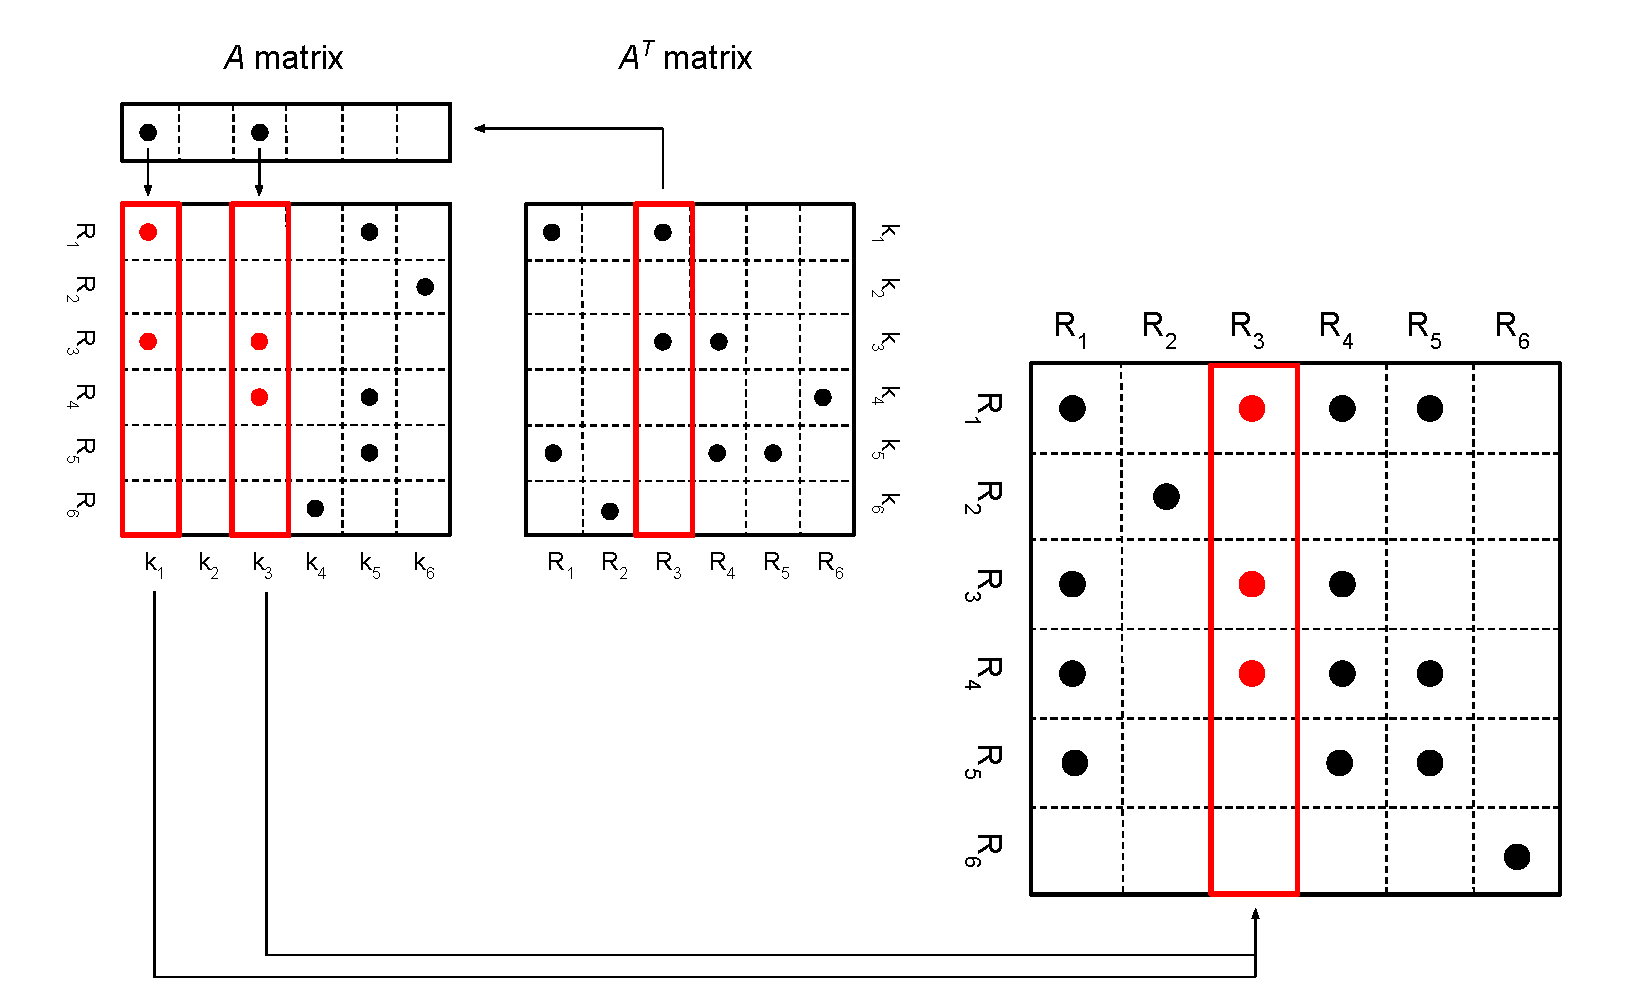
\includegraphics[width=\textwidth]{image/mult.pdf}
    \caption{Sparse matrix multiplication exploiting a $column-by-column$ algorithm \myworries{cite}.}
    \label{fig:mult}
\end{figure}

After that, exploiting the column-by-column algorithm we multiply these two sparse matrices obtaining a resulted matrix, as illustrated in \Cref{fig:mult}.
The final sparse matrix allows us to keep track of all the read pairs that share some k-mers and the corresponding positions on both the reads.
Here, the cell $(i,j)$ consists in a vector containing the k-mers $ids$ are and the corrisponding positions in the read $i$ and read $j$. 
The generality of this approach comes from being able to use the same algorithm to also keep track of distances between shared k-mers. 
In fact, we are interested in keeping track of the distance between shared k-mers as it can provide more evidence of overlap.

To detect which reads pairs show some evidence of potential overlap, we implemented the following method, \Cref{fig:detect}. 
For each read pairs, (a) we compute the distance between each pair of consecutive k-mers both on read $i$ and read $j$.
For each k-mers pairs, (b) we select the shortest distance between the one on read $i$ and on read $j$ and then, given the probabilities of insertion and deletion (that are given by the sequencer), (c) we compute the maximum length of the shortest one (dividing with $1-p_{deletion}$) and the minimum length of the longest one (dividing with $1+p_{insertion}$).
If the former is greater than the latter, we consider that k-mers pair as evidence of potential overlap.
In order to be as conservative as possible and be sure to remove just those reads pairs that certainly not overlap, we decide to keep into account all the reads pairs that present at least one evidence of potential overlap among their k-mers pairs.
\begin{figure}
    \centering
    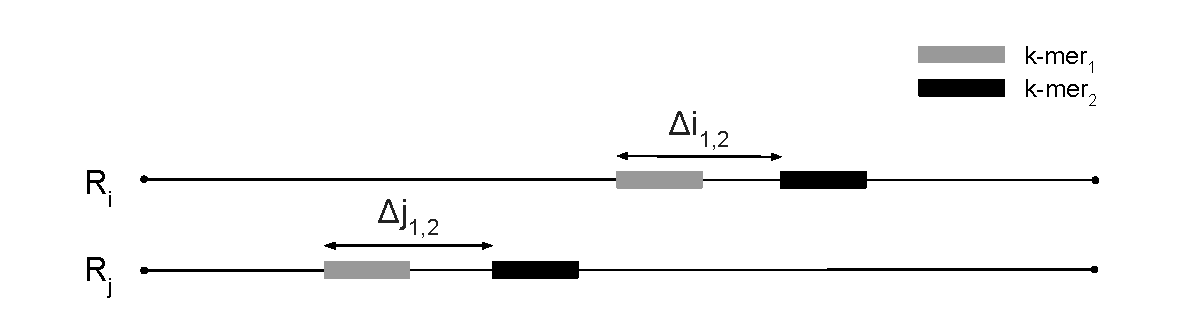
\includegraphics[width=\textwidth]{image/detect.pdf}
    \caption{Reads pair sharing two k-mers.}
    \label{fig:detect}
\end{figure}

\subsection{Evaluation}
\begin{figure}
    \centering
    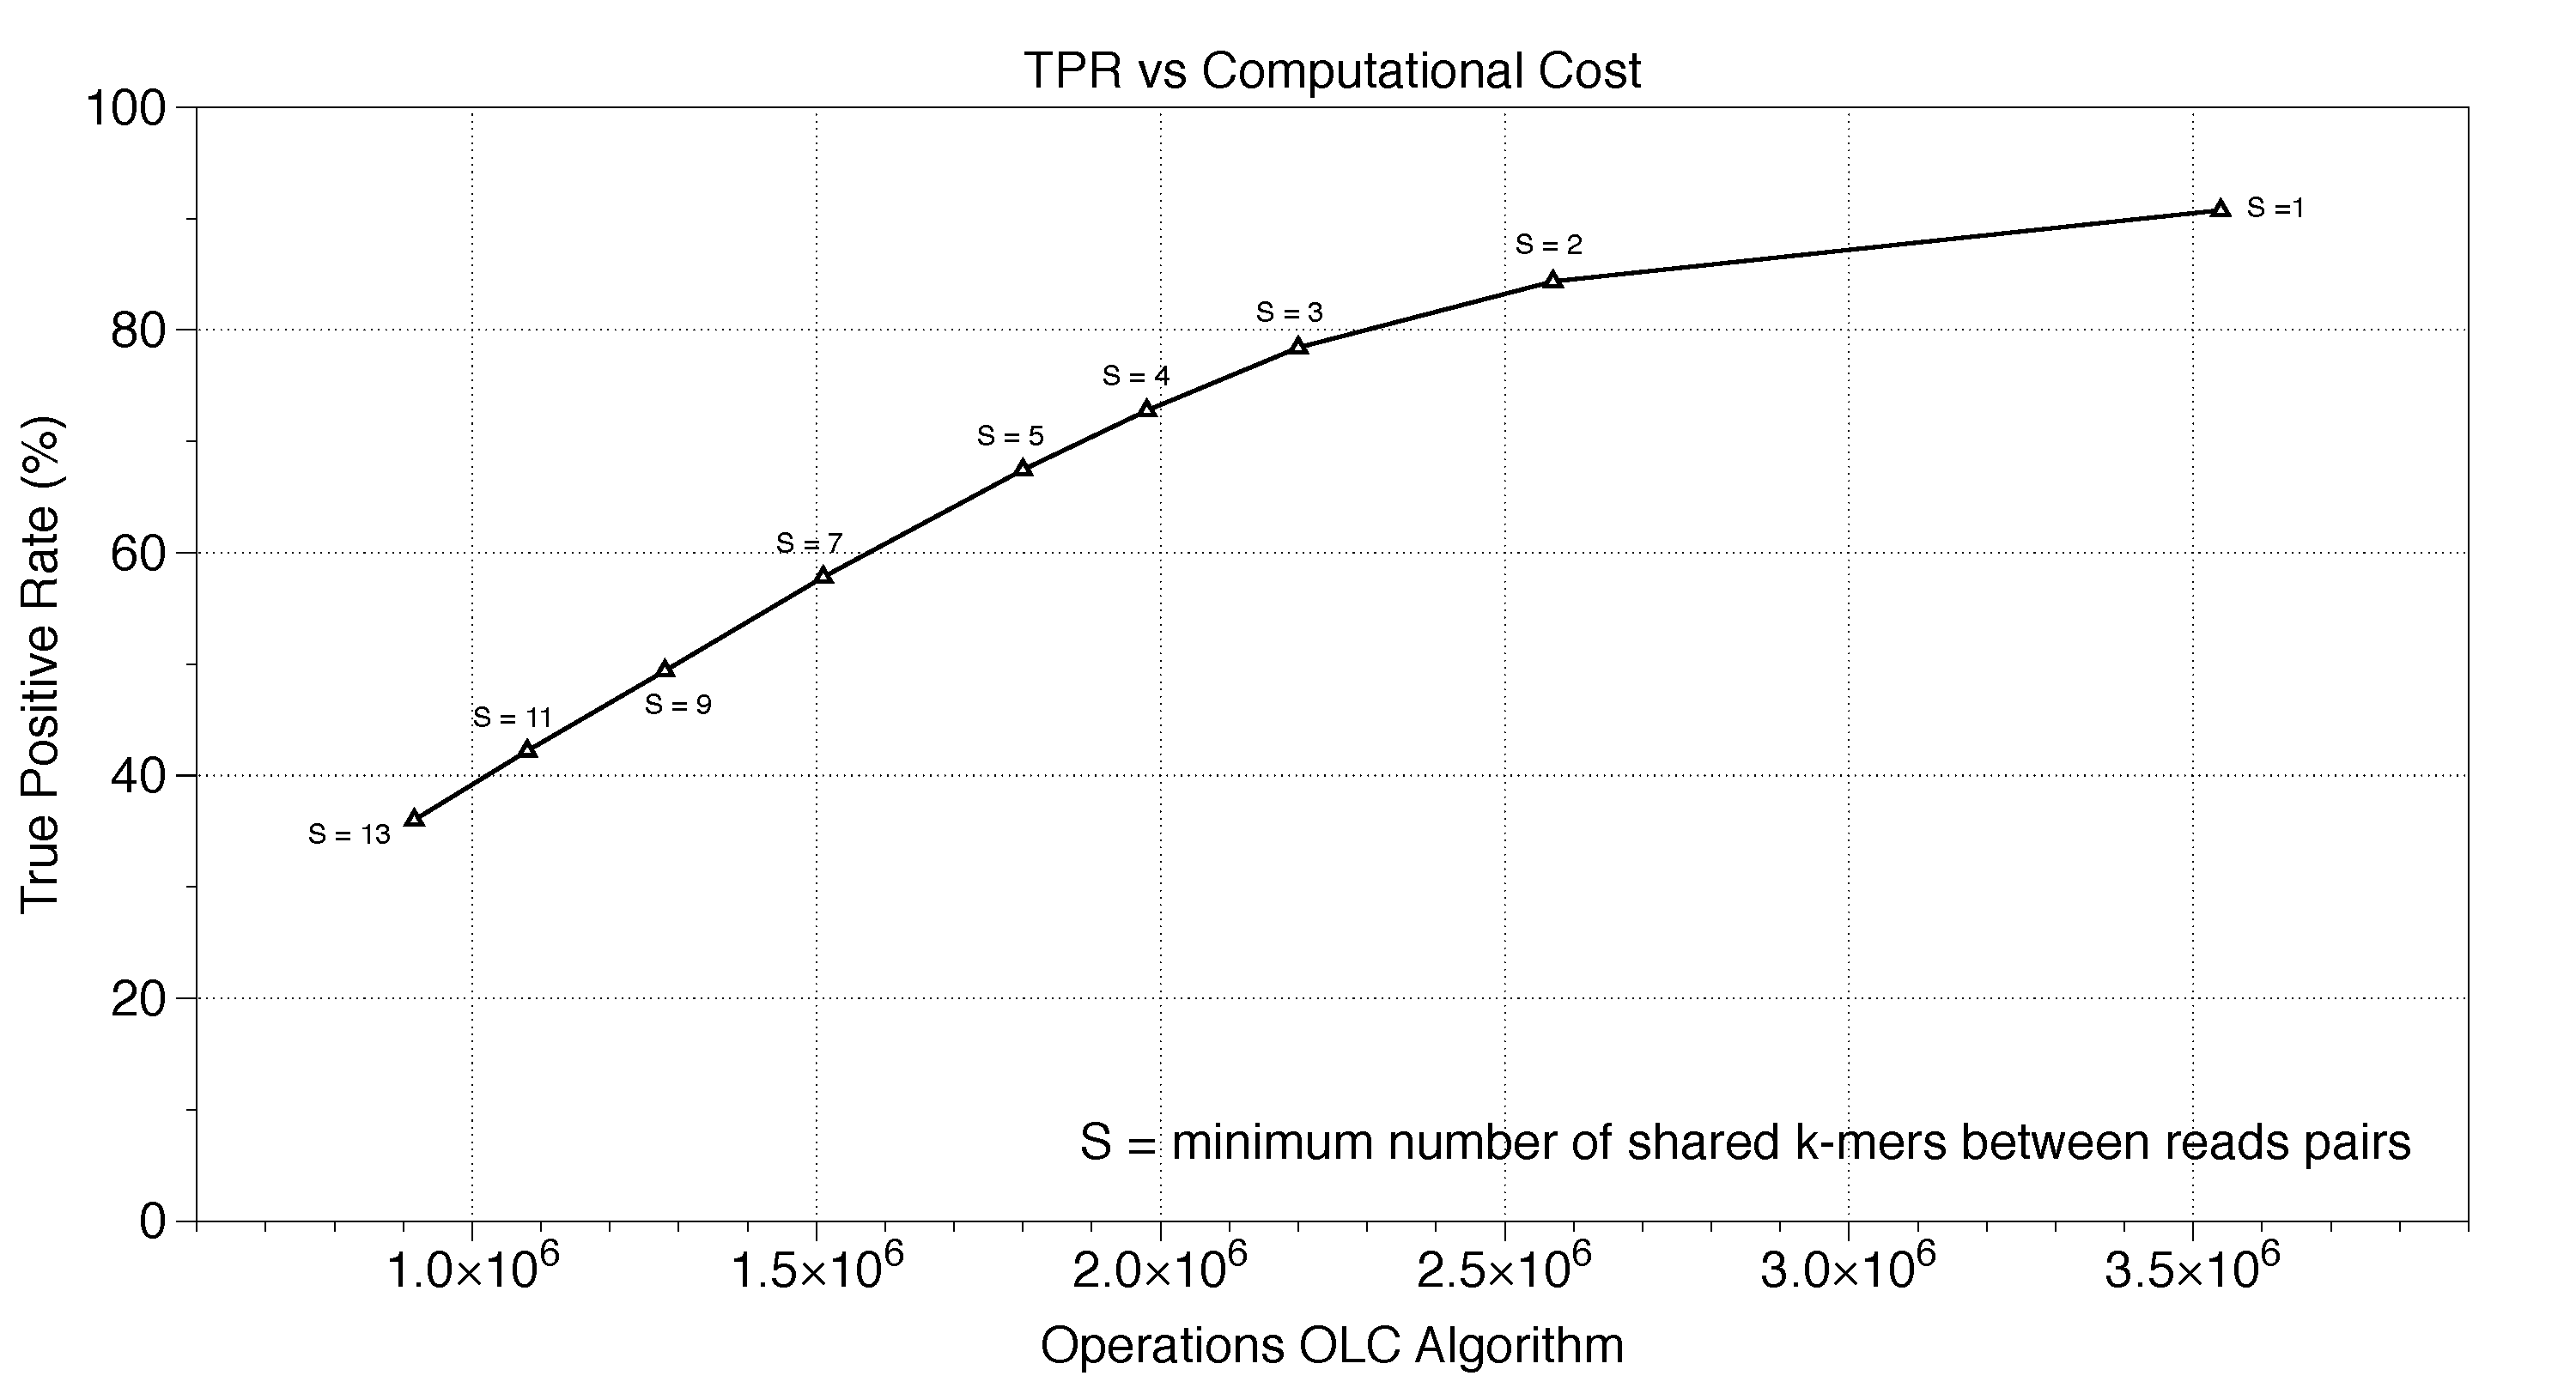
\includegraphics[width=\textwidth]{image/true.pdf}
    \caption{True positive rate compared to the computational cost of the $Overlap-Layout-Consensus$ (OLC) algorithm, the $x$-axis is in log scale.}
    \label{fig:true}
\end{figure}
\begin{figure}
    \centering
    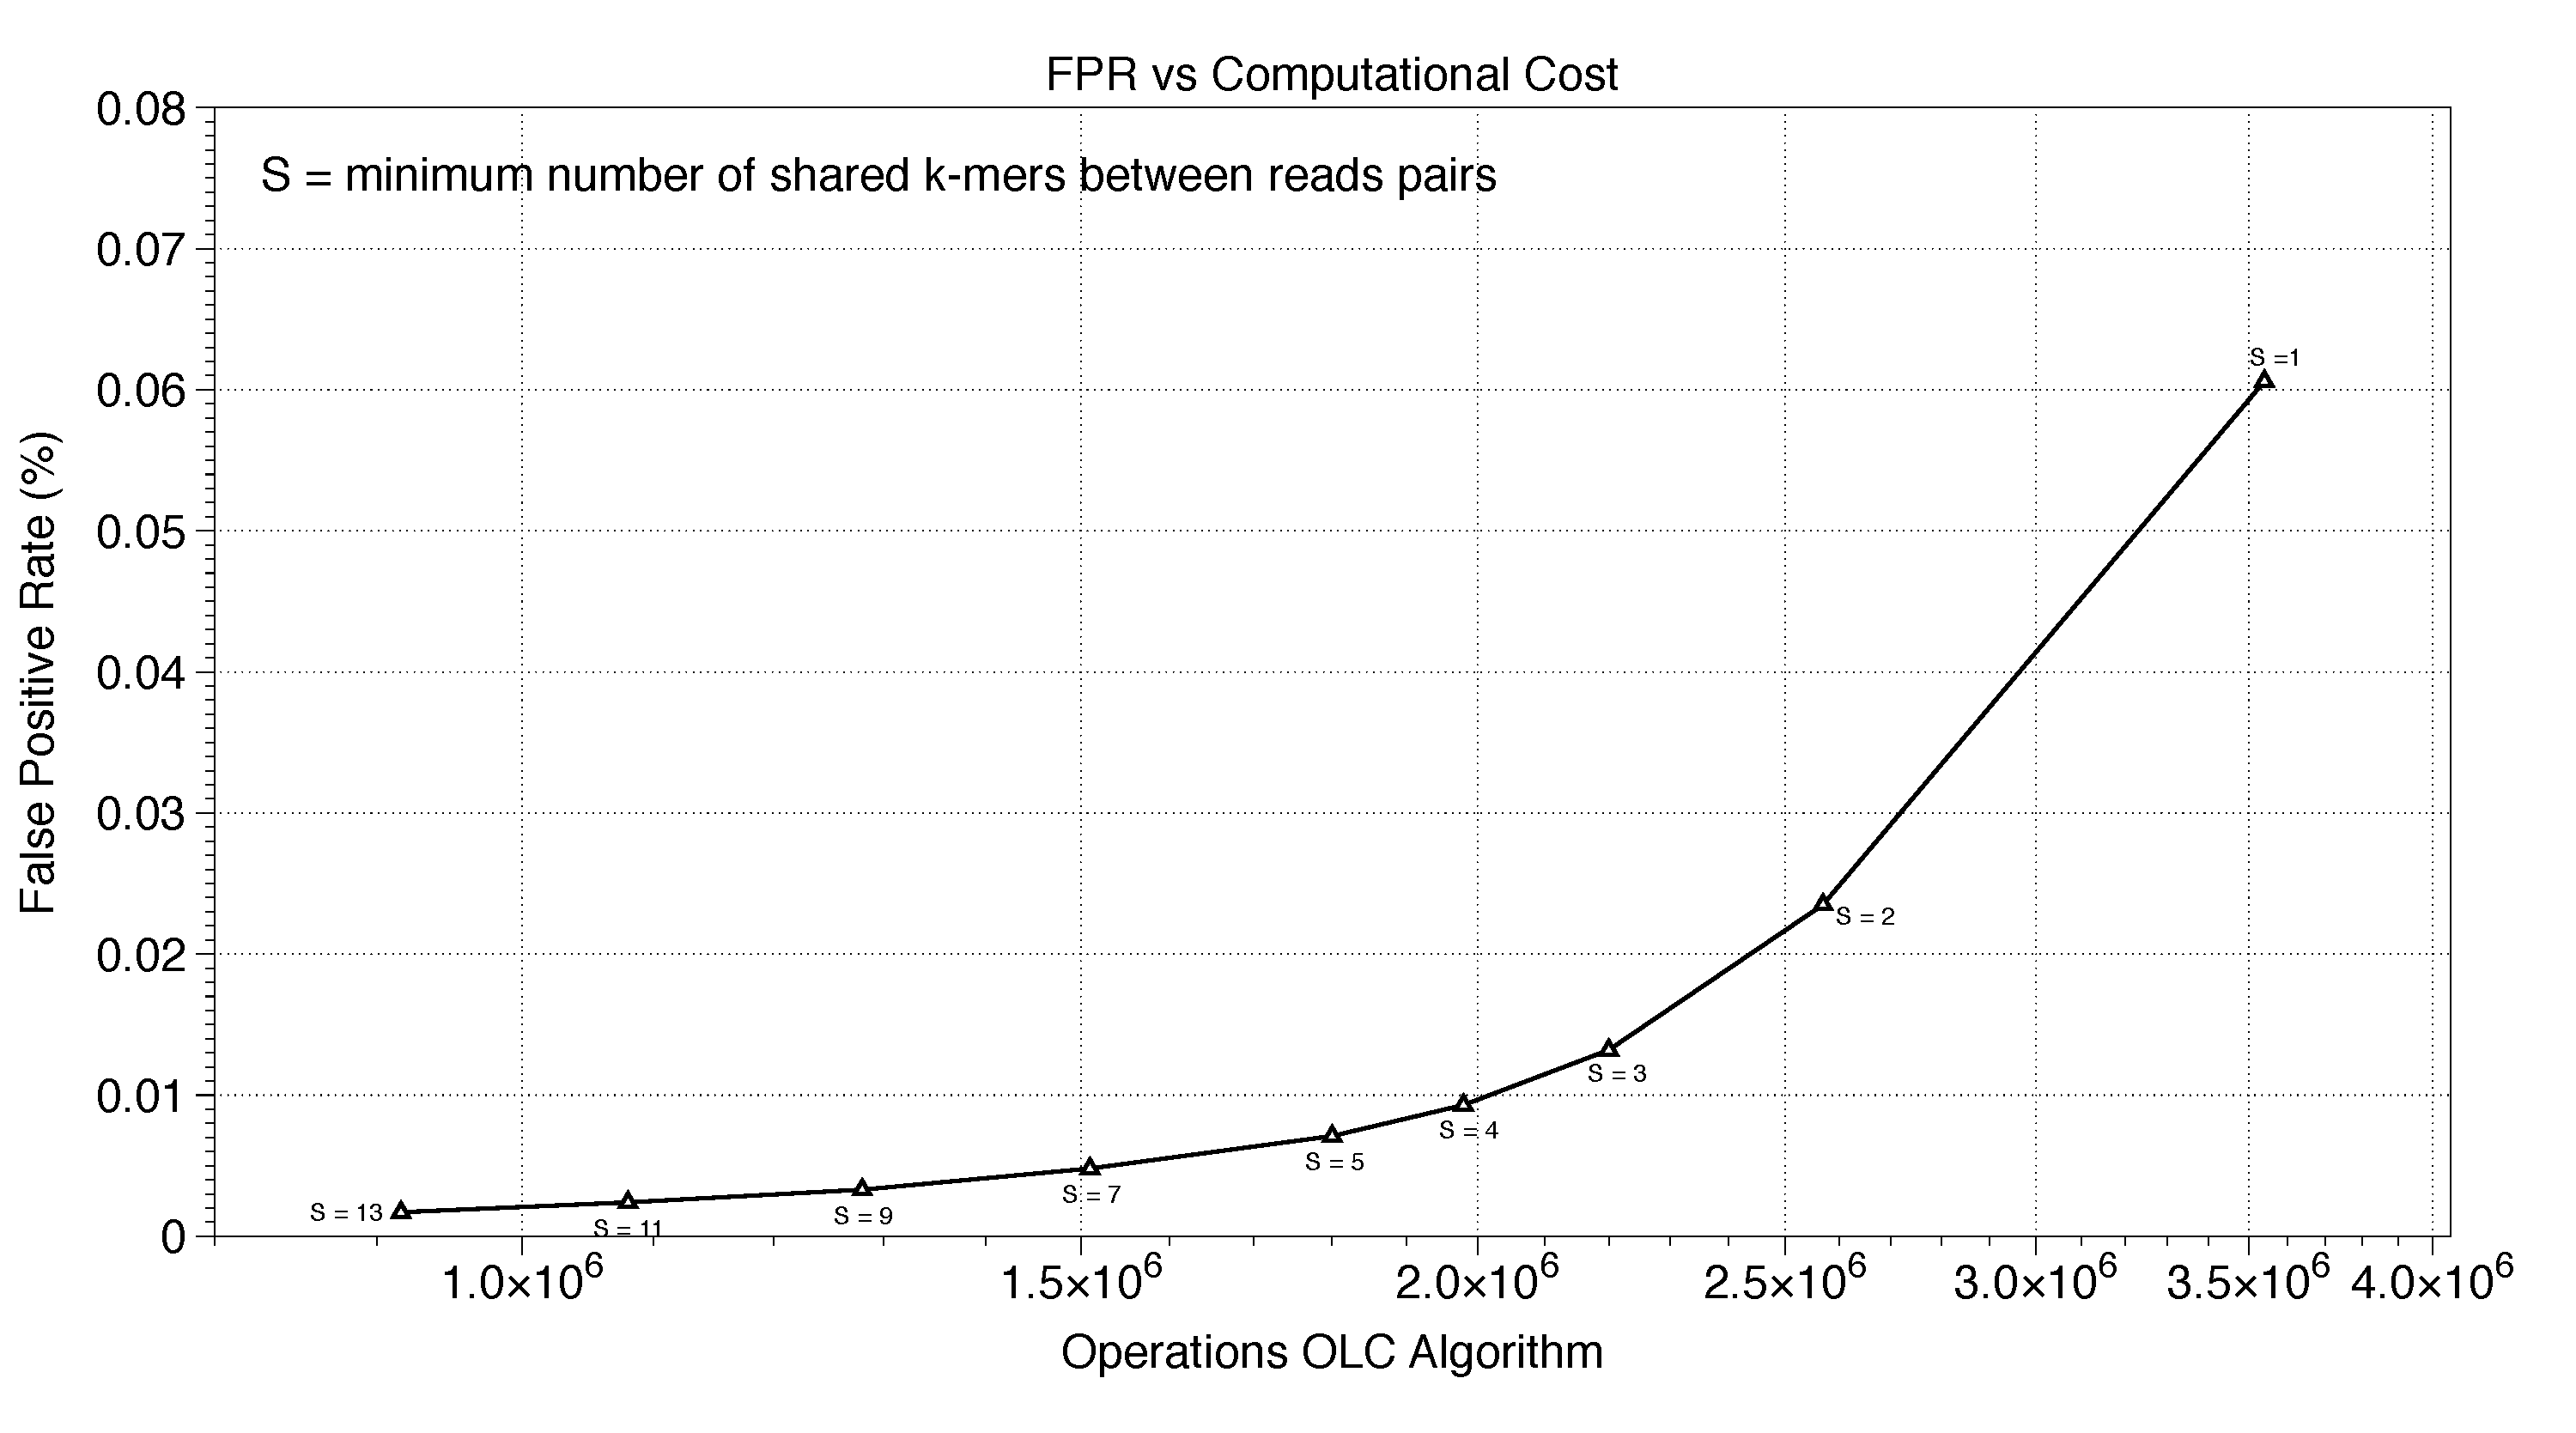
\includegraphics[width=\textwidth]{image/false.pdf}
    \caption{False positive rate compared to the computational cost of the $Overlap-Layout-Consensus$ (OLC) algorithm, the $x$-axis is in log scale.}
    \label{fig:false}
\end{figure}
\begin{figure}
    \centering
    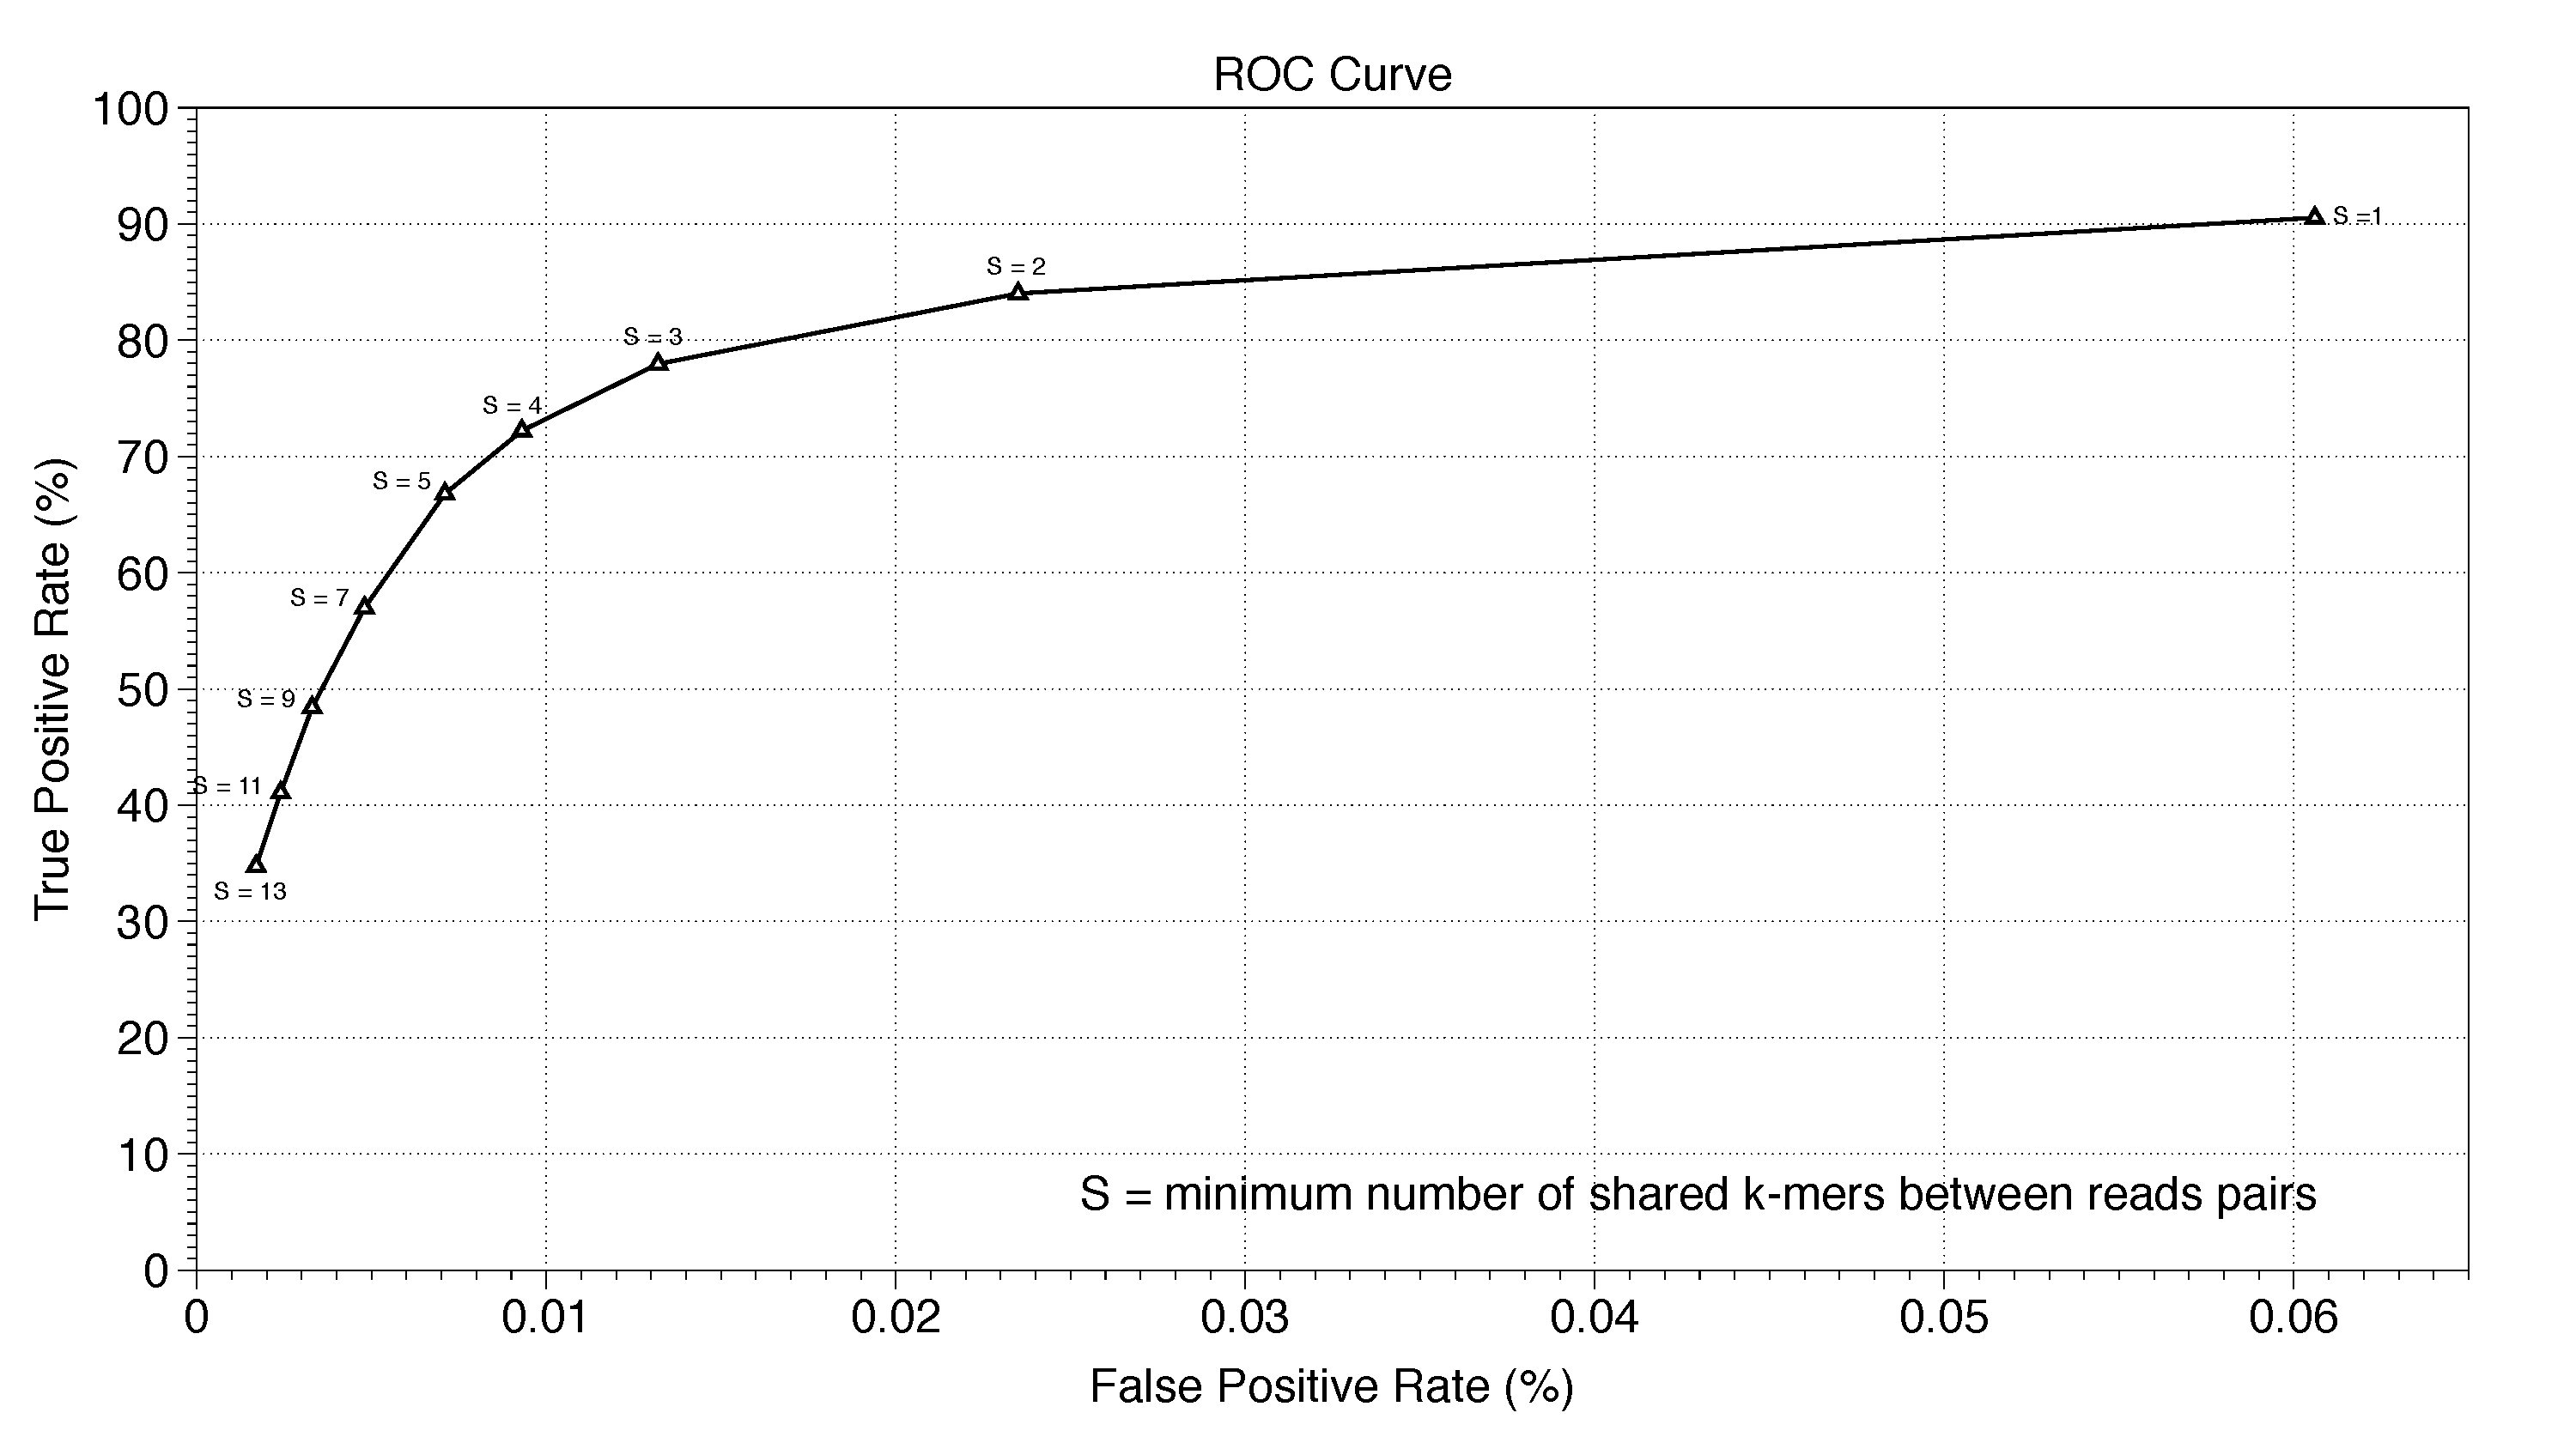
\includegraphics[width=\textwidth]{image/roc.pdf}
    \caption{Receiver Operating Characteristic (ROC) curve.}
    \label{fig:roc}
\end{figure}
To evaluate our approach we measured the true positive rate as measure of the proportion of positives that are correctly identified as such, that means as the ratio between the number of true overlapping reads pairs we detected and actual number of true overlapping pairs.
The false positive rate is calculated as the ratio between the number of non-overlapping reads pairs identified as true overlapping reads pairs (that means the false positives derived from our approach) the total number of actual non-overlapping reads pairs in the entire set of reads.
Both the true positive rate and the false positive one were related to the computational cost of the overlap-layout-consensus algorithm that as a time complexity equal to $O(R)$ where $R$ is the number of reads pairs (\Cref{fig:true} and \Cref{fig:false}), and finally compared to each other through a Receiver Operating Characteristic (ROC) curve curve as shown in \Cref{fig:roc}.
In the plots, the parameter $S$ represents the minimum number of shared k-mers that two reads share.

We see from the plots that, in the most conservative case than means $S$ = 1, our approach achieve a true positive rate of about 91\%.
In later stages, we could exploit transitivity between reads pairs to detect the missing pairs. 
For instance, two reads could be interconnected through a k-mer excluded from the reliable range.
%Firsly, our approach consists in the creation of a dictionary containing all the k-mers belonging to the defined range.
%Then, we construct a [kmer -by- read] sparse matrix, where the ${\{i,j\}}$ cell is a $pair$ data structure.
%The first value of the pair correspond to the identification number of the k-mer $i$ contained in the read $j$, while the second value is a $vector$ data structure where all the positions of that k-mer in the considered read are saved.\\
%Once creating the matrix, we compute its transpose [read -by- k-mer] in order to multiply them and obtain a [read -by- read] matrix.
%We implement the calculation to obtain as final cell ${\{i,j\}}$ a $map$ data structure organized as follow.
%The $keys$ correspond to the identification numbers of the shared k-mers between the two reads, while the $values$ are pairs of vectors containing the k-mers positions on the two reads.\\
%\myworries{To do: filter on the matrix to identify reads pairs sampled from the same region of the genome, implement an Apply() function to compute the delta-pos among k-mers belonging to the same read and compare k-mers delta-pos between reads sharing the same k-mers.}
%Filter to identify \emph{true overlap} reads pair:
%\begin{itemize}
%    \item Compute the delta-pos among k-mers belonging to the same read.
%    \item Comparing k-mers delta-pos between reads sharing the same k-mers.
%    \item If at least one of the comparing is rejected by our filter, we %discharge the considered pair.
%    \item The filter consist in a parametric analysis that takes into account %the probability of indention and deletion (from the PacBio simulator) to %calculate the minimum and maximum length of the two given delta length.
%    \item If there is not overlap between the $L_{max}$ of the shortest read %and the $L_{min}$ of the longest one, the pair is rejected as considered a %\emph{fake overlap}.
%\end{itemize}

\subsection{Light version}

The previous explained version of the algorithm is implemented on single node and it has very high memory requirements. 
%Due to the memory bound, this version does not allow us to test our approach with genomes greater than the \emph{Escherischia Coli} one.
Consequently, we decided to implement a \emph{light} version of the algorithm.
In this second version, the cell $(i,j)$ of the matrices before the multiplication contains the integer value that represents the k-mer $id$ in the k-mers dictionary and the first position of that k-mer in the corresponding read; while the cell $(i,j)$ in the resulted matrix contains three integer values. 
The first represents the number of shared k-mers between the two considered reads, while the second and the third are the positions of the first shared k-mer on the two reads.
%This change allowed us to test our approch with different genomes, as shown in \Cref{table:ram}.
%\begin{table}
%\centering
%\begin{tabular*}{\textwidth}{l @{\extracolsep{\fill}} rrr}
%\hline %inserts double horizontal lines 
%\addlinespace[1ex] Genome & Sequence size (MB) & Reliable k-mers (million) & RAM Usage (GB) \\ 
%%heading
%\addlinespace[1ex]\hline % inserts single horizontal line
%\addlinespace[0.8ex] $E.$ $Coli$ & 4.7 & 1.63 & 1.3 \\ 
%\addlinespace[0.8ex] $C.$ $Elegans$ Chr. $3$ & 14.1 & 4.97 & 7.6 \\
%\addlinespace[0.8ex] $C.$ $Elegans$ Chr. $4$ & 17.8 & 6.87 & 8.3 \\
%\addlinespace[0.8ex] $E.$ $Caballus$ Chr. $31$ & 25.5 & 16.17 & 8.8 \\
%\addlinespace[1ex]\hline
%\end{tabular*}
%\caption{Reliable k-mers and RAM usage of the $light$ algorithm for different genomes.}
%\label{table:ram}
%\end{table}
These changes make infeasible applying the distances filter previously described, as it needs additional information, such as the positions of all the shared k-mers in the reads.
However, we saw that removing the filter does not change significantly our TPR (called also sensitivity) and precision.
The simple selection of reliable k-mers and the application of the sparse matrix multiplication guarantee the best results (that means almost the same maximum we were able to achieve with the previous version of the algorithm) both for sensitivity and precision.
%The sensivity and precision for different genomes are shown in \Cref{table:met}.

\myworries{Work in progress.} To increase our precision, we exploit the information about the first shared k-mer position as it allows us to compute the potential overlap length $L_{ov}$ between two reads, as shown in \Cref{fig:ovlen}.
Following, this length can be used to compute the theoretical maximum edit distance used during the expensive local alignment phase to throw away false positives read pairs.
\begin{figure}
    \centering
    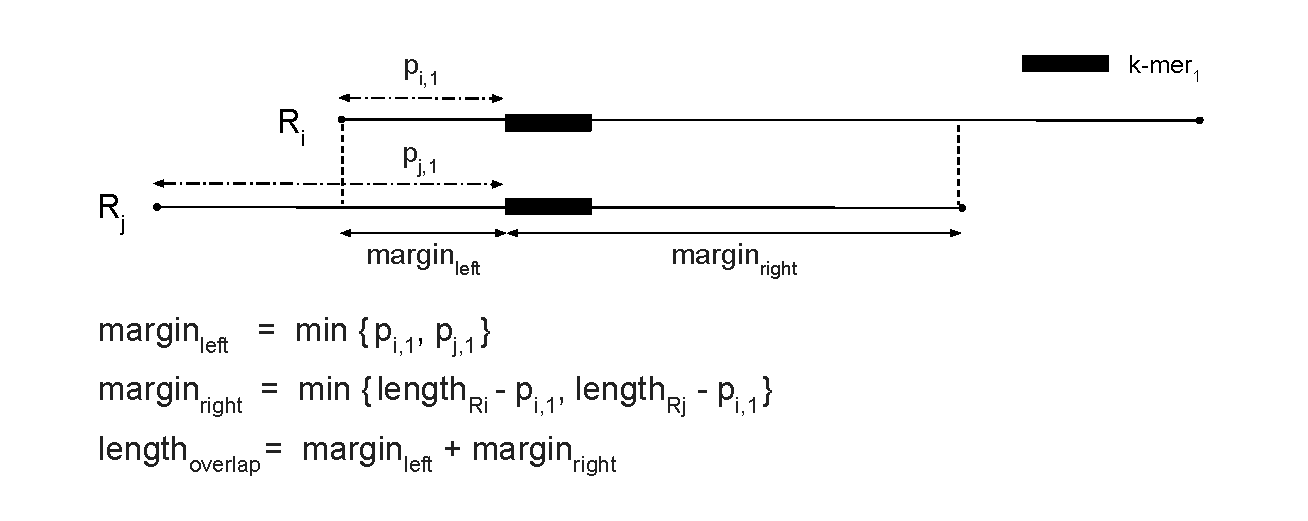
\includegraphics[width=\textwidth]{image/Ovlen.pdf}
    \caption{Overlap length computed exploiting the position of the first shared k-mer between the two considered reads.}
    \label{fig:ovlen}
\end{figure}
If the probability of correctly sequence a bases-pair is equal to $p^2$ where $p=(1-e)$, the average number of correct bases-pairs in a region of length $L_{ov}$ is $\mu = L_{ov} \cdot p^2$, while the standard deviation is $\sigma = \sqrt{L_{ov}\cdot p^2 \cdot (1-p^2)}$.
If we consider our data as normally distributed, we can approximate the maximum edit distance for a given $L_{ov}$, which is computed runtime for each reads pair, as:
$$edit~distance = L_{ov}-L_{ov}\cdot p^2+2\cdot\sqrt{L_{ov}\cdot p^2\cdot (1-p^2)} = L_{ov}-(\mu-2\sigma)$$

So far, knowing that about 95\% of the values drawn from a normal distribution are within $two$ standard deviation $\sigma$ away from the mean, we consider as suitable values those within $2\sigma$.
To sum up, first of all, we compute the number of shared k-mers between two reads exploiting the multiplication.
Then, we apply the local alignment and write on file only those reads pairs which show an edit distance smaller than the one described above.

That said, we can make some further considerations: (a) the precision of our data is significantly better if we consider reads pairs sharing more than $two$ k-mers and (b) the current approach leads to throw away some $true~positive~data$ due to the fact that the k-mer position we use to compute $L_{ov}$ could be wrong.
Consequently, we could decide to apply the local alignment filter only on reads pairs sharing $one$ k-mer. 
In this way for the $Escherichia~Coli$ genome, we would obtain a recall equal to 87.24\% and a precision of 80.33\%.
These percentages show, respectively, a decrease of 3.89\% (before local alignment the recall was 90.77\%) and an increase of 28.36\% (previous precision equal to 62.58\%).
Empirically, moving from $2\sigma$ to $3~or~4\sigma$ in the previous formula does not improve the metrics: the recall remains basically unchanged, while the precision decreases.
That makes sense from a theorically point of view as well, as incrementing the distance from the mean we are prone to cosinder as $true~positive$ erroneous pairs.
\myworries{Think about how to improve these percentages, perhaps a correction factor while computing $L_{ov}$.}
%In the MECAT paper (http://www.biorxiv.org/content/early/2016/12/15/089250), the authors consider just reads with length at %least equal to 5000 bp (Figure 2 in their paper) and define that two reads has the correct pairwise relationship if they %overlap for more than 2000 bp (Table 2 in their paper).
%So, we generated the initial set of reads with pbsim setting 5000 bp as minimum length and setting the threshold to consider %a pair as correct (both in the initial set and when we filter our pairs) equal to 2000 bp.
%In this case, for instance for the $E.Coli$, we obtain a recall of 99\% and a precision of 34\%. 
%Even if the precision is lower with respect to our previous implementation, the number of reads pairs on which compute the %local alignment is smaller (about 1.23 millions less than before, but we're still wasting a lot of computation).
%Considering than in a region of length 2000, we expected to see about 8 shared k-mers (computed as $2000 \cdot (1-e)^{34}$), %setting 4 as minimum number of shared k-mers to be more conservative, we obtain 98.14\% of recall and 68.6\% of precision, %setting 8 we got 93.94\% of recall and 78.8\% of precision.
%The results obtained applying MECAT thresholds for difference genomes are reported in \Cref{table:mecat}.
%The term \emph{computational saving} in \Cref{table:mecat} is defined as $1-\frac{TP+FP}{R^2}$, where TP are the true %positives, FP are the false positives and R is number of reads.
%
%\begin{table}
%\centering
%\begin{tabular}{lrr}
%\hline %inserts double horizontal lines 
%\addlinespace[1ex] Genome & Sensitivity (\%) & Precision (\%) \\ 
%%heading
%\addlinespace[1ex]\hline % inserts single horizontal line
%\addlinespace[0.8ex] $E.$ $Coli$ & 90.77 & 62.58 \\ 
%\addlinespace[0.8ex] $C.$ $Elegans$ Chr. $3$ & 91.14 & 3.80 \\
%\addlinespace[0.8ex] $C.$ $Elegans$ Chr. $4$ & 91.53 & 3.50 \\
%\addlinespace[0.8ex] $E.$ $Caballus$ Chr. $31$ & 94.16 & 5.91 \\
%\addlinespace[1ex]\hline
%\end{tabular}
%\caption{$Light$ version: sensitivity and precision for different genomes.}
%\label{table:met}
%\end{table}
%
%\begin{table}
%\centering
%\begin{tabular*}{\textwidth}{l @{\extracolsep{\fill}} rrr}
%\hline %inserts double horizontal lines 
%\addlinespace[1ex]Genome & Sensitivity (\%) & Precision (\%) & Computational saving (\%) \\ 
%%heading
%\addlinespace[1ex]\hline % inserts single horizontal line
%\addlinespace[0.8ex] $E.$ $Coli$ & 98.15 & 68.60 & 99.68 \\ 
%\addlinespace[0.8ex] $C.$ $Elegans$ Chr. $3$ & 97.67 & 30.25 & 99.76 \\
%\addlinespace[0.8ex] $C.$ $Elegans$ Chr. $4$ & 97.89 & 31.06 & 99.81 \\
%\addlinespace[0.8ex] $E.$ $Caballus$ Chr. $31$ & 98.94 & 16.83 & 99.76 \\
%\addlinespace[1ex]\hline
%\addlinespace[0.8ex] $E.$ $Coli$ & 93.94 & 78.87 & 99.74 \\ 
%\addlinespace[0.8ex] $C.$ $Elegans$ Chr. $3$ & 92.26 & 73.04 & 99.91 \\
%\addlinespace[0.8ex] $C.$ $Elegans$ Chr. $4$ & 92.80 & 70.79 & 99.92 \\
%\addlinespace[0.8ex] $E.$ $Caballus$ Chr. $31$ & 96.13 & 31.89 & 99.88 \\
%\addlinespace[1ex]\hline
%\end{tabular*}
%\caption{$Light$ version: sensitivity and precision for different genomes computed using MECAT threshold (minimum read %length = 5000 bp and minimum overlap = 2000 bp) with number of shared k-mers $S$ equal to 4 (upper part of the table) and 8 (%lower part).}
%\label{table:mecat}
%\end{table}

\clearpage

%\appendix
%\section{Tables}\label{append}
%
%\begin{longtable}{r|r|r|r|r|r}
%\caption{Existence and Unique existence of 15-mers}\\
%\toprule
%\textbf{GroupID} & \textbf{State A} & \textbf{State B} & \textbf{State C} & \%textbf{Existence (\%)} & \textbf{Unique existence (\%)}\\
%\midrule
%\endhead
%    2     & 11054964 & 1163913 & 6137  & 9.57 & 9.52 \\
%    3     & 2067194 & 828871 & 8706  & 28.83 & 28.53 \\
%    4     & 630466 & 455824 & 9450  & 42.46 & 41.60 \\
%    5     & 230524 & 207638 & 8646  & 48.41 & 46.47 \\
%    6     & 83858 & 83304 & 6986  & 51.85 & 47.84 \\
%    7     & 29699 & 30686 & 5231  & 54.74 & 46.77 \\
%    8     & 10289 & 11145 & 4045  & 59.62 & 43.74 \\
%    9     & 3953  & 4078  & 3081  & 64.43 & 36.70 \\
%    10    & 1621  & 1555  & 2756  & 72.67 & 26.21 \\
%    11    & 847   & 681   & 2466  & 78.79 & 17.05 \\
%    12    & 456   & 364   & 2161  & 84.70 & 12.21 \\
%    13    & 285   & 162   & 1941  & 88.07 & 6.78 \\
%    14    & 217   & 84    & 1684  & 89.07 & 4.23 \\
%    15    & 158   & 43    & 1321  & 89.62 & 2.83 \\
%    16    & 106   & 27    & 1148  & 91.73 & 2.11 \\
%    17    & 79    & 18    & 901   & 92.08 & 1.80 \\
%    18    & 79    & 21    & 708   & 90.22 & 2.60 \\
%    19    & 55    & 15    & 534   & 90.89 & 2.48 \\
%    20    & 49    & 12    & 462   & 90.63 & 2.29 \\
%    21    & 47    & 6     & 356   & 88.51 & 1.47 \\
%    22    & 34    & 12    & 301   & 90.20 & 3.46 \\
%    23    & 39    & 4     & 242   & 86.32 & 1.40 \\
%    24    & 29    & 7     & 204   & 87.92 & 2.92 \\
%    25    & 19    & 4     & 176   & 90.45 & 2.01 \\
%    26    & 18    & 3     & 157   & 89.89 & 1.69 \\
%    27    & 11    & 5     & 153   & 93.49 & 2.96 \\
%    28    & 13    & 4     & 98    & 88.70 & 3.48 \\
%    29    & 13    & 8     & 87    & 87.96 & 7.41 \\
%    30    & 13    & 4     & 67    & 84.52 & 4.76 \\
%    31    & 9     & 2     & 52    & 85.71 & 3.17 \\
%    32    & 11    & 1     & 36    & 77.08 & 2.08 \\
%    33    & 7     & 0     & 34    & 82.93 & 0.00 \\
%    34    & 6     & 4     & 24    & 82.35 & 11.76 \\
%    35    & 0     & 3     & 26    & 100.00 & 10.34 \\
%    36    & 6     & 2     & 11    & 68.42 & 10.53 \\
%    37    & 5     & 1     & 6     & 58.33 & 8.33 \\
%    38    & 6     & 1     & 9     & 62.50 & 6.25 \\
%    39    & 5     & 0     & 9     & 64.29 & 0.00 \\
%    40    & 1     & 0     & 8     & 88.89 & 0.00 \\
%    41    & 3     & 0     & 8     & 72.73 & 0.00 \\
%    42    & 2     & 1     & 10    & 84.62 & 7.69 \\
%    43    & 3     & 0     & 4     & 57.14 & 0.00 \\
%    44    & 2     & 1     & 7     & 80.00 & 10.00 \\
%    45    & 0     & 0     & 6     & 100.00 & 0.00 \\
%    46    & 2     & 1     & 5     & 75.00 & 12.50 \\
%    47    & 1     & 1     & 4     & 83.33 & 16.67 \\
%    48    & 0     & 0     & 4     & 100.00 & 0.00 \\
%    49    & 1     & 0     & 5     & 83.33 & 0.00\\
%    50    & 2     & 0     & 3     & 60.00 & 0.00\\
%    51    & 1     & 0     & 4     & 80.00 & 0.00\\
%    53    & 1     & 0     & 9     & 90.00 & 0.00\\
%    54    & 1     & 0     & 2     & 66.67 & 0.00\\
%    56    & 0     & 0     & 1     & 100.00 & 0.00 \\
%    57    & 0     & 0     & 5     & 100.00 & 0.00 \\
%    58    & 0     & 0     & 3     & 100.00 & 0.00 \\
%    59    & 0     & 0     & 4     & 100.00 & 0.00 \\
%    60    & 0     & 0     & 1     & 100.00 & 0.00 \\
%    62    & 0     & 0     & 2     & 100.00 & 0.00 \\
%    63    & 0     & 0     & 3     & 100.00 & 0.00 \\
%    64    & 0     & 0     & 1     & 100.00 & 0.00 \\
%    65    & 0     & 0     & 1     & 100.00 & 0.00 \\
%    66    & 0     & 0     & 1     & 100.00 & 0.00 \\
%    67    & 0     & 0     & 1     & 100.00 & 0.00 \\
%    68    & 0     & 0     & 1     & 100.00 & 0.00 \\
%    69    & 0     & 0     & 1     & 100.00 & 0.00 \\
%    72    & 0     & 0     & 1     & 100.00 & 0.00 \\
%    74    & 0     & 0     & 2     & 100.00 & 0.00 \\
%    75    & 0     & 0     & 1     & 100.00 & 0.00 \\
%    77    & 0     & 0     & 1     & 100.00 & 0.00 \\
%    79    & 0     & 0     & 1     & 100.00 & 0.00 \\
%    80    & 0     & 0     & 3     & 100.00 & 0.00 \\
%    81    & 0     & 0     & 1     & 100.00 & 0.00 \\
%    83    & 0     & 0     & 1     & 100.00 & 0.00 \\
%    84    & 0     & 0     & 1     & 100.00 & 0.00 \\
%    85    & 0     & 0     & 2     & 100.00 & 0.00 \\
%    86    & 0     & 0     & 1     & 100.00 & 0.00 \\
%    87    & 0     & 0     & 1     & 100.00 & 0.00 \\
%    88    & 0     & 0     & 1     & 100.00 & 0.00 \\
%    90    & 0     & 0     & 3     & 100.00 & 0.00 \\
%    92    & 0     & 0     & 1     & 100.00 & 0.00 \\
%    93    & 0     & 0     & 2     & 100.00 & 0.00 \\
%    94    & 0     & 0     & 1     & 100.00 & 0.00 \\
%    97    & 0     & 0     & 1     & 100.00 & 0.00 \\
%    98    & 0     & 0     & 2     & 100.00 & 0.00 \\
%    99    & 0     & 0     & 2     & 100.00 & 0.00 \\
%    100   & 0     & 0     & 3     & 100.00 & 0.00 \\
%    101   & 0     & 0     & 2     & 100.00 & 0.00 \\
%    102   & 0     & 0     & 2     & 100.00 & 0.00 \\
%    103   & 0     & 0     & 2     & 100.00 & 0.00 \\
%    105   & 0     & 0     & 1     & 100.00 & 0.00 \\
%    106   & 0     & 0     & 1     & 100.00 & 0.00 \\
%    108   & 0     & 0     & 1     & 100.00 & 0.00 \\
%    109   & 0     & 0     & 2     & 100.00 & 0.00 \\
%    111   & 0     & 0     & 1     & 100.00 & 0.00 \\
%    114   & 0     & 0     & 1     & 100.00 & 0.00 \\
%    115   & 0     & 0     & 1     & 100.00 & 0.00 \\
%    116   & 0     & 0     & 1     & 100.00 & 0.00 \\
%    117   & 0     & 0     & 3     & 100.00 & 0.00 \\
%    118   & 0     & 0     & 3     & 100.00 & 0.00 \\
%    121   & 0     & 0     & 1     & 100.00 & 0.00 \\
%    122   & 0     & 0     & 5     & 100.00 & 0.00 \\
%    123   & 0     & 0     & 3     & 100.00 & 0.00 \\
%    124   & 0     & 0     & 1     & 100.00 & 0.00 \\
%    125   & 0     & 0     & 1     & 100.00 & 0.00 \\
%    126   & 0     & 0     & 3     & 100.00 & 0.00 \\
%    127   & 0     & 0     & 3     & 100.00 & 0.00 \\
%    128   & 0     & 0     & 4     & 100.00 & 0.00 \\
%    129   & 0     & 0     & 4     & 100.00 & 0.00 \\
%    130   & 0     & 0     & 1     & 100.00 & 0.00 \\
%    132   & 0     & 0     & 2     & 100.00 & 0.00 \\
%    133   & 0     & 0     & 1     & 100.00 & 0.00 \\
%    134   & 0     & 0     & 1     & 100.00 & 0.00 \\
%    135   & 0     & 0     & 1     & 100.00 & 0.00 \\
%    137   & 0     & 0     & 2     & 100.00 & 0.00 \\
%    138   & 0     & 0     & 4     & 100.00 & 0.00 \\
%    139   & 0     & 0     & 1     & 100.00 & 0.00 \\
%    140   & 0     & 0     & 1     & 100.00 & 0.00 \\
%    141   & 0     & 0     & 1     & 100.00 & 0.00 \\
%    143   & 0     & 0     & 1     & 100.00 & 0.00 \\
%    144   & 0     & 0     & 1     & 100.00 & 0.00 \\
%    145   & 0     & 0     & 2     & 100.00 & 0.00 \\
%    146   & 0     & 0     & 1     & 100.00 & 0.00 \\
%    148   & 0     & 0     & 1     & 100.00 & 0.00 \\
%    152   & 0     & 0     & 1     & 100.00 & 0.00 \\
%    156   & 0     & 0     & 1     & 100.00 & 0.00 \\
%    157   & 0     & 0     & 3     & 100.00 & 0.00 \\
%    158   & 0     & 0     & 2     & 100.00 & 0.00 \\
%    159   & 0     & 0     & 4     & 100.00 & 0.00 \\
%    161   & 0     & 0     & 1     & 100.00 & 0.00 \\
%    163   & 0     & 0     & 1     & 100.00 & 0.00 \\
%    164   & 0     & 0     & 2     & 100.00 & 0.00 \\
%    166   & 0     & 0     & 2     & 100.00 & 0.00 \\
%    168   & 0     & 0     & 2     & 100.00 & 0.00 \\
%    169   & 0     & 0     & 1     & 100.00 & 0.00 \\
%    171   & 0     & 0     & 2     & 100.00 & 0.00 \\
%    173   & 0     & 0     & 1     & 100.00 & 0.00 \\
%    179   & 0     & 0     & 1     & 100.00 & 0.00 \\
%    182   & 0     & 0     & 1     & 100.00 & 0.00 \\
%    183   & 0     & 0     & 2     & 100.00 & 0.00 \\
%    185   & 0     & 0     & 1     & 100.00 & 0.00 \\
%    186   & 0     & 0     & 1     & 100.00 & 0.00 \\
%    190   & 0     & 0     & 1     & 100.00 & 0.00 \\
%    191   & 0     & 0     & 3     & 100.00 & 0.00 \\
%    192   & 0     & 0     & 1     & 100.00 & 0.00 \\
%    198   & 0     & 0     & 1     & 100.00 & 0.00 \\
%    199   & 0     & 0     & 1     & 100.00 & 0.00 \\
%    201   & 0     & 0     & 2     & 100.00 & 0.00 \\
%    202   & 0     & 0     & 1     & 100.00 & 0.00 \\
%    205   & 0     & 0     & 1     & 100.00 & 0.00 \\
%    208   & 0     & 0     & 1     & 100.00 & 0.00 \\
%    210   & 0     & 0     & 1     & 100.00 & 0.00 \\
%    212   & 0     & 0     & 1     & 100.00 & 0.00 \\
%    219   & 0     & 0     & 1     & 100.00 & 0.00 \\
%    220   & 0     & 0     & 1     & 100.00 & 0.00 \\
%    221   & 0     & 0     & 1     & 100.00 & 0.00 \\
%    232   & 0     & 0     & 1     & 100.00 & 0.00 \\
%    261   & 0     & 0     & 1     & 100.00 & 0.00 \\
%    268   & 0     & 0     & 1     & 100.00 & 0.00 \\
%    \bottomrule
%\end{longtable} 
%
%\begin{longtable}{r|r|r|r|r|r} 
%\caption{Existence and Unique existence of 17-mers}\\
%\toprule
%\textbf{GroupID} & \textbf{State A} & \textbf{State B} & \textbf{State C} & \%textbf{Existence (\%)} & \textbf{Unique existence (\%)}\\
%\midrule
%\endhead
%    2     & 3652095 & 1099555 & 3952  & 23.20 & 23.12 \\
%    3     & 668265 & 529021 & 4477  & 44.39 & 44.02 \\
%    4     & 206144 & 194009 & 3977  & 48.99 & 48.01 \\
%    5     & 60569 & 58288 & 3571  & 50.53 & 47.61 \\
%    6     & 16525 & 14935 & 3104  & 52.19 & 43.21 \\
%    7     & 4352  & 3505  & 2774  & 59.06 & 32.97 \\
%    8     & 1419  & 872   & 2673  & 71.41 & 17.57 \\
%    9     & 612   & 289   & 2537  & 82.20 & 8.41 \\
%    10    & 335   & 111   & 2327  & 87.92 & 4.00 \\
%    11    & 207   & 68    & 1983  & 90.83 & 3.01 \\
%    12    & 137   & 50    & 1704  & 92.76 & 2.64 \\
%    13    & 81    & 37    & 1319  & 94.36 & 2.57 \\
%    14    & 65    & 11    & 1045  & 94.20 & 0.98 \\
%    15    & 60    & 16    & 777   & 92.97 & 1.88 \\
%    16    & 42    & 10    & 594   & 93.50 & 1.55 \\
%    17    & 35    & 8     & 417   & 92.39 & 1.74 \\
%    18    & 31    & 4     & 284   & 90.28 & 1.25 \\
%    19    & 25    & 2     & 245   & 90.81 & 0.74 \\
%    20    & 17    & 7     & 156   & 90.56 & 3.89 \\
%    21    & 13    & 2     & 88    & 87.38 & 1.94 \\
%    22    & 13    & 2     & 75    & 85.56 & 2.22 \\
%    23    & 5     & 5     & 55    & 92.31 & 7.69 \\
%    24    & 8     & 1     & 25    & 76.47 & 2.94 \\
%    25    & 3     & 2     & 19    & 87.50 & 8.33 \\
%    26    & 3     & 0     & 15    & 83.33 & 0.00 \\
%    27    & 0     & 0     & 11    & 100.00 & 0.00 \\
%    28    & 4     & 0     & 14    & 77.78 & 0.00 \\
%    29    & 1     & 0     & 11    & 91.67 & 0.00 \\
%    30    & 0     & 1     & 11    & 100.00 & 8.33 \\
%    31    & 1     & 0     & 9     & 90.00 & 0.00 \\
%    32    & 1     & 0     & 1     & 50.00 & 0.00 \\
%    33    & 1     & 0     & 5     & 83.33 & 0.00 \\
%    34    & 0     & 0     & 7     & 100.00 & 0.00 \\
%    35    & 0     & 0     & 3     & 100.00 & 0.00 \\
%    36    & 0     & 0     & 6     & 100.00 & 0.00 \\
%    37    & 0     & 0     & 2     & 100.00 & 0.00 \\
%    38    & 0     & 0     & 1     & 100.00 & 0.00 \\
%    39    & 1     & 0     & 4     & 80.00 & 0.00 \\
%    40    & 0     & 0     & 2     & 100.00 & 0.00 \\
%    41    & 0     & 0     & 2     & 100.00 & 0.00 \\
%    42    & 0     & 0     & 2     & 100.00 & 0.00 \\
%    43    & 0     & 0     & 4     & 100.00 & 0.00 \\
%    44    & 0     & 0     & 3     & 100.00 & 0.00 \\
%    45    & 0     & 0     & 1     & 100.00 & 0.00 \\
%    46    & 0     & 0     & 3     & 100.00 & 0.00 \\
%    47    & 0     & 0     & 3     & 100.00 & 0.00 \\
%    48    & 0     & 0     & 1     & 100.00 & 0.00 \\
%    50    & 0     & 0     & 4     & 100.00 & 0.00 \\
%    51    & 0     & 0     & 4     & 100.00 & 0.00 \\
%    53    & 0     & 0     & 4     & 100.00 & 0.00 \\
%    54    & 0     & 0     & 4     & 100.00 & 0.00 \\
%    57    & 0     & 0     & 3     & 100.00 & 0.00 \\
%    58    & 0     & 0     & 2     & 100.00 & 0.00 \\
%    59    & 0     & 0     & 3     & 100.00 & 0.00 \\
%    60    & 0     & 0     & 2     & 100.00 & 0.00 \\
%    61    & 0     & 0     & 4     & 100.00 & 0.00 \\
%    63    & 0     & 0     & 5     & 100.00 & 0.00 \\
%    64    & 0     & 0     & 2     & 100.00 & 0.00 \\
%    65    & 0     & 0     & 2     & 100.00 & 0.00 \\
%    66    & 0     & 0     & 1     & 100.00 & 0.00 \\
%    68    & 0     & 0     & 2     & 100.00 & 0.00 \\
%    69    & 0     & 0     & 1     & 100.00 & 0.00 \\
%    70    & 0     & 0     & 1     & 100.00 & 0.00 \\
%    71    & 0     & 0     & 6     & 100.00 & 0.00 \\
%    72    & 0     & 0     & 1     & 100.00 & 0.00 \\
%    74    & 0     & 0     & 1     & 100.00 & 0.00 \\
%    75    & 0     & 0     & 1     & 100.00 & 0.00 \\
%    76    & 0     & 0     & 1     & 100.00 & 0.00 \\
%    77    & 0     & 0     & 5     & 100.00 & 0.00 \\
%    79    & 0     & 0     & 3     & 100.00 & 0.00 \\
%    80    & 0     & 0     & 4     & 100.00 & 0.00 \\
%    81    & 0     & 0     & 1     & 100.00 & 0.00 \\
%    82    & 0     & 0     & 5     & 100.00 & 0.00 \\
%    83    & 0     & 0     & 1     & 100.00 & 0.00 \\
%    84    & 0     & 0     & 2     & 100.00 & 0.00 \\
%    85    & 0     & 0     & 6     & 100.00 & 0.00 \\
%    86    & 0     & 0     & 5     & 100.00 & 0.00 \\
%    87    & 0     & 0     & 1     & 100.00 & 0.00 \\
%    89    & 0     & 0     & 1     & 100.00 & 0.00 \\
%    90    & 0     & 0     & 1     & 100.00 & 0.00 \\
%    91    & 0     & 0     & 2     & 100.00 & 0.00 \\
%    92    & 0     & 0     & 1     & 100.00 & 0.00 \\
%    94    & 0     & 0     & 1     & 100.00 & 0.00 \\
%    95    & 0     & 0     & 1     & 100.00 & 0.00 \\
%    98    & 0     & 0     & 1     & 100.00 & 0.00 \\
%    100   & 0     & 0     & 2     & 100.00 & 0.00 \\
%    101   & 0     & 0     & 2     & 100.00 & 0.00 \\
%    104   & 0     & 0     & 3     & 100.00 & 0.00 \\
%    106   & 0     & 0     & 1     & 100.00 & 0.00 \\
%    107   & 0     & 0     & 1     & 100.00 & 0.00 \\
%    108   & 0     & 0     & 1     & 100.00 & 0.00 \\
%    109   & 0     & 0     & 1     & 100.00 & 0.00 \\
%    110   & 0     & 0     & 1     & 100.00 & 0.00 \\
%    112   & 0     & 0     & 1     & 100.00 & 0.00 \\
%    114   & 0     & 0     & 1     & 100.00 & 0.00 \\
%    116   & 0     & 0     & 1     & 100.00 & 0.00 \\
%    118   & 0     & 0     & 1     & 100.00 & 0.00 \\
%    120   & 0     & 0     & 1     & 100.00 & 0.00 \\
%    122   & 0     & 0     & 1     & 100.00 & 0.00 \\
%    125   & 0     & 0     & 2     & 100.00 & 0.00 \\
%    127   & 0     & 0     & 1     & 100.00 & 0.00 \\
%    130   & 0     & 0     & 1     & 100.00 & 0.00 \\
%    136   & 0     & 0     & 3     & 100.00 & 0.00 \\
%    140   & 0     & 0     & 2     & 100.00 & 0.00 \\
%    141   & 0     & 0     & 1     & 100.00 & 0.00 \\
%    143   & 0     & 0     & 1     & 100.00 & 0.00 \\
%    151   & 0     & 0     & 1     & 100.00 & 0.00 \\
%    153   & 0     & 0     & 1     & 100.00 & 0.00 \\
%    164   & 0     & 0     & 1     & 100.00 & 0.00 \\
%    166   & 0     & 0     & 1     & 100.00 & 0.00 \\
%    \bottomrule
%\end{longtable}
%
%\begin{longtable}{r|r|r|r|r|r} 
%\caption{Existence and Unique existence of 19-mers}\\
%\toprule
%\textbf{GroupID} & \textbf{State A} & \textbf{State B} & \textbf{State C} & \%textbf{Existence (\%)} & \textbf{Unique existence (\%)}\\
%\midrule
%\endhead
%    2     & 2089009 & 868637 & 4796  & 29.48 & 29.32 \\
%    3     & 363543 & 307174 & 4804  & 46.18 & 45.47 \\
%    4     & 88917 & 81730 & 4402  & 49.20 & 46.69 \\
%    5     & 20364 & 17910 & 3813  & 51.61 & 42.55 \\
%    6     & 4305  & 3883  & 3282  & 62.47 & 33.85 \\
%    7     & 1150  & 732   & 2801  & 75.44 & 15.63 \\
%    8     & 410   & 175   & 2182  & 85.18 & 6.32 \\
%    9     & 197   & 59    & 1765  & 90.25 & 2.92 \\
%    10    & 123   & 27    & 1218  & 91.01 & 1.97 \\
%    11    & 57    & 15    & 897   & 94.12 & 1.55 \\
%    12    & 42    & 15    & 718   & 94.58 & 1.94 \\
%    13    & 23    & 8     & 490   & 95.59 & 1.54 \\
%    14    & 20    & 13    & 352   & 94.81 & 3.38 \\
%    15    & 17    & 5     & 268   & 94.14 & 1.72 \\
%    16    & 9     & 4     & 176   & 95.24 & 2.12 \\
%    17    & 4     & 2     & 122   & 96.88 & 1.56 \\
%    18    & 2     & 8     & 82    & 97.83 & 8.70 \\
%    19    & 3     & 0     & 51    & 94.44 & 0.00 \\
%    20    & 6     & 1     & 43    & 88.00 & 2.00 \\
%    21    & 3     & 0     & 24    & 88.89 & 0.00 \\
%    22    & 2     & 0     & 20    & 90.91 & 0.00 \\
%    23    & 1     & 0     & 10    & 90.91 & 0.00 \\
%    24    & 0     & 0     & 6     & 100.00 & 0.00 \\
%    25    & 1     & 0     & 5     & 83.33 & 0.00 \\
%    26    & 0     & 0     & 5     & 100.00 & 0.00 \\
%    27    & 1     & 0     & 2     & 66.67 & 0.00 \\
%    28    & 1     & 0     & 3     & 75.00 & 0.00 \\
%    29    & 0     & 0     & 4     & 100.00 & 0.00 \\
%    30    & 0     & 0     & 4     & 100.00 & 0.00 \\
%    31    & 0     & 0     & 6     & 100.00 & 0.00 \\
%    32    & 1     & 0     & 1     & 50.00 & 0.00 \\
%    33    & 1     & 0     & 3     & 75.00 & 0.00 \\
%    34    & 0     & 0     & 1     & 100.00 & 0.00 \\
%    35    & 0     & 0     & 1     & 100.00 & 0.00 \\
%    36    & 0     & 0     & 1     & 100.00 & 0.00 \\
%    37    & 0     & 0     & 3     & 100.00 & 0.00 \\
%    38    & 0     & 0     & 5     & 100.00 & 0.00 \\
%    40    & 0     & 0     & 6     & 100.00 & 0.00 \\
%    41    & 0     & 0     & 1     & 100.00 & 0.00 \\
%    42    & 0     & 0     & 3     & 100.00 & 0.00 \\
%    43    & 0     & 0     & 3     & 100.00 & 0.00 \\
%    44    & 0     & 0     & 5     & 100.00 & 0.00 \\
%    45    & 0     & 0     & 5     & 100.00 & 0.00 \\
%    46    & 0     & 0     & 4     & 100.00 & 0.00 \\
%    47    & 0     & 0     & 5     & 100.00 & 0.00 \\
%    48    & 0     & 0     & 2     & 100.00 & 0.00 \\
%    49    & 0     & 0     & 2     & 100.00 & 0.00 \\
%    50    & 0     & 0     & 4     & 100.00 & 0.00 \\
%    51    & 0     & 0     & 3     & 100.00 & 0.00 \\
%    52    & 0     & 0     & 3     & 100.00 & 0.00 \\
%    53    & 0     & 0     & 3     & 100.00 & 0.00 \\
%    54    & 0     & 0     & 2     & 100.00 & 0.00 \\
%    56    & 0     & 0     & 2     & 100.00 & 0.00 \\
%    57    & 0     & 0     & 3     & 100.00 & 0.00 \\
%    58    & 0     & 0     & 1     & 100.00 & 0.00 \\
%    59    & 0     & 0     & 4     & 100.00 & 0.00 \\
%    60    & 0     & 0     & 3     & 100.00 & 0.00 \\
%    61    & 0     & 0     & 3     & 100.00 & 0.00 \\
%    62    & 0     & 0     & 2     & 100.00 & 0.00 \\
%    63    & 0     & 0     & 3     & 100.00 & 0.00 \\
%    64    & 0     & 0     & 2     & 100.00 & 0.00 \\
%    66    & 0     & 0     & 2     & 100.00 & 0.00 \\
%    67    & 0     & 0     & 2     & 100.00 & 0.00 \\
%    76    & 0     & 0     & 1     & 100.00 & 0.00 \\
%    77    & 0     & 0     & 2     & 100.00 & 0.00 \\
%    78    & 0     & 0     & 1     & 100.00 & 0.00 \\
%    79    & 0     & 0     & 2     & 100.00 & 0.00 \\
%    80    & 0     & 0     & 2     & 100.00 & 0.00 \\
%    81    & 0     & 0     & 1     & 100.00 & 0.00 \\
%    86    & 0     & 0     & 1     & 100.00 & 0.00 \\
%    87    & 0     & 0     & 1     & 100.00 & 0.00 \\
%    88    & 0     & 0     & 1     & 100.00 & 0.00 \\
%    89    & 0     & 0     & 1     & 100.00 & 0.00 \\
%    92    & 0     & 0     & 2     & 100.00 & 0.00 \\
%    93    & 0     & 0     & 4     & 100.00 & 0.00 \\
%    103   & 0     & 0     & 1     & 100.00 & 0.00 \\
%    105   & 0     & 0     & 1     & 100.00 & 0.00 \\
%    106   & 0     & 0     & 2     & 100.00 & 0.00 \\
%    118   & 0     & 0     & 1     & 100.00 & 0.00 \\
%    \bottomrule
%\end{longtable}

\bibliographystyle{abbrv}
\bibliography{report}

\end{document}